\documentclass[dvipsnames, aspectratio=169]{beamer}
\usepackage[utf8]{inputenc}
\usepackage{listings}
\usepackage{comment}
\usepackage{soul}
%\usepackage{ulem}
\usepackage{subfig}
\usepackage{pgf-pie}
\setul{}{1pt}
\usepackage[oldenum, olditem]{paralist}
%allow even smaller text
\newcommand\tinytiny{\fontsize{4pt}{3}\selectfont}

\makeatletter
\let\old@lstKV@SwitchCases\lstKV@SwitchCases
\def\lstKV@SwitchCases#1#2#3{}
\makeatother
\usepackage{lstlinebgrd}
\makeatletter
\let\lstKV@SwitchCases\old@lstKV@SwitchCases

\lst@Key{numbers}{none}{%
    \def\lst@PlaceNumber{\lst@linebgrd}%
    \lstKV@SwitchCases{#1}%
    {none:\\%
     left:\def\lst@PlaceNumber{\llap{\normalfont
                \lst@numberstyle{\thelstnumber}\kern\lst@numbersep}\lst@linebgrd}\\%
     right:\def\lst@PlaceNumber{\rlap{\normalfont
                \kern\linewidth \kern\lst@numbersep
                \lst@numberstyle{\thelstnumber}}\lst@linebgrd}%
    }{\PackageError{Listings}{Numbers #1 unknown}\@ehc}}
\makeatother


%disclaimer for Sandia. uncomment and the whole blob goes away @ b80c116300122
\def\sandid{SAND2020-8766 PE}
\usepackage{pgfplotstable}

% \title{Performance Portability with Kokkos}
\title{The Kokkos Lectures}

%BAD misuse of author field
\author{Module 6: Fortran/Python interoperability, MPI and PGAS}

%\author{
%  Jeff Miles \inst{1},
%  Christian Trott \inst{1}
%  Jan Ciesko \inst{1}
%}
%\institute[shortinst]{\tiny \inst{1} Sandia National Laboratories, \inst{2} Oak Ridge National Laboratory \and \inst{3} Los Alamos National Laboratory}
%\institute[shortinst]{\tiny \inst{1} Sandia National Laboratories}

\usetheme{kokkos}

\newif\ifshort
\newif\ifmedium
\newif\iffull
\newif\ifnotoverview

\newcommand{\TutorialDirectory}{\texttt{Intro-Full}}
\newcommand{\ExerciseDirectory}[1]{\texttt{Exercises/#1/}}
\newcommand{\TutorialClone}{\texttt{Kokkos/kokkos-tutorials/\TutorialDirectory}}

\definecolor{darkgreen}{rgb}{0.0, 0.5, 0.0}
\definecolor{darkred}{rgb}{0.8, 0.0, 0.0}
\definecolor{orange}{rgb}{0.8, 0.33, 0.0}
\definecolor{purple}{rgb}{0.60, 0.20, 0.80}
\colorlet{bodyColor}{blue!20}
\colorlet{patternColor}{orange!30}
\colorlet{policyColor}{green!30}

% http://tex.stackexchange.com/questions/144448/color-a-text-line-in-a-code-lstlisting
\lstnewenvironment{code}[1][]%
{
  %with txfonts: OT1/txr/m/n/10
  %with default fonts: OT1/cmr/m/n/10
  %\fontfamily{cmr}\selectfont
  %\showthe\font
   \noindent
   \minipage{\linewidth}
   %\vspace{0.5\baselineskip}
   \lstset{mathescape, escapeinside={<@}{@>},
moredelim=**[is][{\btHL[fill=patternColor]}]{@pattern}{@pattern},
moredelim=**[is][{\btHL[fill=red!30]}]{@warning}{@warning},
moredelim=**[is][{\btHL[fill=policyColor]}]{@policy}{@policy},
moredelim=**[is][{\btHL[fill=bodyColor]}]{@body}{@body},
moredelim=**[is][{\btHL[fill=red!30]}]{@warning}{@warning},
moredelim=**[is][\color{black}]{@black}{@black},
moredelim=**[is][\color{blue}]{@blue}{@blue},
moredelim=**[is][\bf]{@bold}{@bold},
moredelim=**[is][\it]{@italic}{@italic},
moredelim=**[is][\color{boldblue}\bf]{@boldblue}{@boldblue},
moredelim=**[is][\color{red}]{@red}{@red},
moredelim=**[is][\color{green}]{@green}{@green},
moredelim=**[is][\color{gray}]{@gray}{@gray},
moredelim=**[is][\color{darkgreen}]{@darkgreen}{@darkgreen},
moredelim=**[is][\color{darkred}]{@darkred}{@darkred},
moredelim=**[is][\color{orange}]{@orange}{@orange},
moredelim=**[is][\color{purple}]{@purple}{@purple},
keywords={},
#1}
}
{
  \endminipage
  %\vspace{1.0\baselineskip}
}

\makeatletter
\newif\ifATOlinebackground
\lst@Key{linebackground}{\tiny}{\def\ATOlinebackground{#1}\global\ATOlinebackgroundtrue}
\makeatother

\lstnewenvironment{shell}[1][]{%
  \global\ATOlinebackgroundfalse
  \lstset{language=sh,%
    showstringspaces=false,
    aboveskip=0pt,
    frame=none,
    numbers=none,
    belowskip=2pt,
    breaklines=true,
    #1,
    }
  %\ifATOlinebackground
  \lstset{linebackgroundcolor={
    \ATOlinebackground
  }}
  %\fi
  }{}

\lstnewenvironment{cmake}[1][]{%
  \global\ATOlinebackgroundfalse
  \lstset{language=sh,%
    showstringspaces=false,
    aboveskip=0pt,
    frame=none,
    numbers=none,
    belowskip=2pt,
    breaklines=true,
    #1,
    }
  %\ifATOlinebackground
  \lstset{linebackgroundcolor={
    \ATOlinebackground
  }}
  %\fi
  }{}

\newcommand{\inlinecode}[1]{{\lstset{basicstyle=\ttfamily,keywordstyle={},showstringspaces=false}\lstinline$#1$}}
\newcommand{\inlineshell}[1]{{\lstset{basicstyle=\ttfamily,keywordstyle={},showstringspaces=false}\lstinline$#1$}}

\setbeamercolor{block title}{fg=white, bg=SandiaLightBlue}
\setbeamercolor{block body}{bg=lightgray}
\setbeamercolor{block title alerted}{fg=white, bg=SandiaRed}
\setbeamercolor{block body alerted}{bg=lightgray}



%\usepackage[texcoord,grid,gridunit=mm,gridcolor=red!10,subgridcolor=green!10]{eso-pic}
\usepackage[absolute,overlay]{textpos}





% http://tex.stackexchange.com/questions/8851/how-can-i-highlight-some-lines-from-source-code

\usepackage{pgf, pgffor}
\usepackage{listings}
\usepackage{lstlinebgrd} % see http://www.ctan.org/pkg/lstaddons

\makeatletter
%%%%%%%%%%%%%%%%%%%%%%%%%%%%%%%%%%%%%%%%%%%%%%%%%%%%%%%%%%%%%%%%%%%%%%%%%%%%%%
%
% \btIfInRange{number}{range list}{TRUE}{FALSE}
%
% Test in int number <number> is element of a (comma separated) list of ranges
% (such as: {1,3-5,7,10-12,14}) and processes <TRUE> or <FALSE> respectively

\newcount\bt@rangea
\newcount\bt@rangeb

\newcommand\btIfInRange[2]{%
    \global\let\bt@inrange\@secondoftwo%
    \edef\bt@rangelist{#2}%
    \foreach \range in \bt@rangelist {%
        \afterassignment\bt@getrangeb%
        \bt@rangea=0\range\relax%
        \pgfmathtruncatemacro\result{ ( #1 >= \bt@rangea) && (#1 <= \bt@rangeb) }%
        \ifnum\result=1\relax%
            \breakforeach%
            \global\let\bt@inrange\@firstoftwo%
        \fi%
    }%
    \bt@inrange%
}
\newcommand\bt@getrangeb{%
    \@ifnextchar\relax%
        {\bt@rangeb=\bt@rangea}%
        {\@getrangeb}%
}
\def\@getrangeb-#1\relax{%
    \ifx\relax#1\relax%
        \bt@rangeb=100000%   \maxdimen is too large for pgfmath
    \else%
        \bt@rangeb=#1\relax%
    \fi%
}

%%%%%%%%%%%%%%%%%%%%%%%%%%%%%%%%%%%%%%%%%%%%%%%%%%%%%%%%%%%%%%%%%%%%%%%%%%%%%%
%
% \btLstHL<overlay spec>{range list}
%
% TODO BUG: \btLstHL commands can not yet be accumulated if more than one overlay spec match.
%
\newcommand<>{\btLstHL}[2]{%
  \only#3{\btIfInRange{\value{lstnumber}}{#1}{\color{#2}\def\lst@linebgrdcmd{\color@block}}{\def\lst@linebgrdcmd####1####2####3{}}}%
}%
\makeatother






% http://tex.stackexchange.com/questions/15237/highlight-text-in-code-listing-while-also-keeping-syntax-highlighting
%\usepackage[T1]{fontenc}
%\usepackage{listings,xcolor,beramono}
\usepackage{tikz}

\makeatletter
\newenvironment{btHighlight}[1][]
{\begingroup\tikzset{bt@Highlight@par/.style={#1}}\begin{lrbox}{\@tempboxa}}
{\end{lrbox}\bt@HL@box[bt@Highlight@par]{\@tempboxa}\endgroup}

\newcommand\btHL[1][]{%
  \begin{btHighlight}[#1]\bgroup\aftergroup\bt@HL@endenv%
}
\def\bt@HL@endenv{%
  \end{btHighlight}%
  \egroup
}
\newcommand{\bt@HL@box}[2][]{%
  \tikz[#1]{%
    \pgfpathrectangle{\pgfpoint{1pt}{0pt}}{\pgfpoint{\wd #2}{\ht #2}}%
    \pgfusepath{use as bounding box}%
    \node[anchor=base west, fill=orange!30,outer sep=0pt,inner xsep=1pt, inner ysep=0pt, rounded corners=3pt, minimum height=\ht\strutbox+1pt,#1]{\raisebox{1pt}{\strut}\strut\usebox{#2}};
  }%
}
\makeatother



\usetikzlibrary{calc}
\usepackage{xparse}%  For \NewDocumentCommand

% tikzmark command, for shading over items
\newcommand{\tikzmark}[1]{\tikz[overlay,remember picture] \node (#1) {};}

\makeatletter
\NewDocumentCommand{\DrawBox}{s O{}}{%
    \tikz[overlay,remember picture]{
    \IfBooleanTF{#1}{%
        \coordinate (RightPoint) at ($(left |- right)+(\linewidth-\labelsep-\labelwidth,0.0)$);
    }{%
        \coordinate (RightPoint) at (right.east);
    }%
    \draw[red,#2]
      ($(left)+(-0.2em,0.9em)$) rectangle
      ($(RightPoint)+(0.2em,-0.3em)$);}
}

\NewDocumentCommand{\DrawBoxWide}{s O{}}{%
    \tikz[overlay,remember picture]{
    \IfBooleanTF{#1}{%
        \coordinate (RightPoint) at ($(left |- right)+(\linewidth-\labelsep-\labelwidth,0.0)$);
    }{%
        \coordinate (RightPoint) at (right.east);
    }%
    \draw[red,#2]
      ($(left)+(-\labelwidth,0.9em)$) rectangle
      ($(RightPoint)+(0.2em,-0.3em)$);}
}

\NewDocumentCommand{\DrawBoxWideBlack}{s O{}}{%
    \tikz[overlay,remember picture]{
    \IfBooleanTF{#1}{%
        \coordinate (RightPoint) at ($(left |- right)+(\linewidth-\labelsep-\labelwidth,0.0)$);
    }{%
        \coordinate (RightPoint) at (right.east);
    }%
    \draw[black,#2]
      ($(left)+(-\labelwidth,0.9em)$) rectangle
      ($(RightPoint)+(0.2em,-0.3em)$);}
}
\makeatother

\usetikzlibrary{positioning}

\usetikzlibrary{shapes}

\hypersetup{
    colorlinks=true,
    linkcolor=blue,
    filecolor=magenta,
    urlcolor=cyan,
}



\shortfalse
\mediumtrue
\fulltrue
\notoverviewtrue

\begin{document}

% \begin{frame}
%   \titlepage
% \end{frame}
% 
%==============================================================================

\begin{frame}{NVIDIA's NVLABS LOGISTICS (1)}

\textbf{\large SOFTWARE FOR LAB}

\vspace{10pt}

\textbf{Remote Desktop Software:} \\
\begin{itemize}
\item {Download NoMachine now for best performance from \\
 \textbf{\ul{www.nomachine.com/download}}}
\item {Alternatively you may use a VNC client or the provided browser-based VNC option}
\end{itemize}

\vspace{10pt}

\textbf{SSH Access Software (optional):}
\begin{itemize}
\item PuTTy for Windows can be downloaded from \textbf{\ul{www.putty.org}}
\item{Alternatively you may use a provided browser-based SSH option}
\end{itemize}

\end{frame}

%==============================================================================

\begin{frame}{NVIDIA's NVLABS LOGISTICS (2)}

\textbf{\Large CONNECTION INSTRUCTIONS}
\begin{itemize}
\item {Navigate to \textbf{\ul{nvlabs.qwiklab.com}}}
\item {Login or create a new account}
\item {Select the \textbf{Instructor-Led Hands-on Labs} Class}
\item {Find the lab called \textbf{Kokkos, ...}, select it, click Select, and finally click Start}
\item {After a short wait, lab instance Connection information will be shown}
\item {Please ask Lab Assistants for help!}
\end{itemize}

\end{frame}

%==============================================================================



\begin{frame}
	\titlepage
\end{frame}

\begin{frame}[fragile]{Welcome to Kokkos}

\textbf{Online Resources}:

\begin{itemize}
        \item \url{https://github.com/kokkos}:
                \begin{itemize}
                        \item Primary Kokkos GitHub Organization
                \end{itemize}
        \item \url{https://github.com/kokkos/kokkos-tutorials/wiki/Kokkos-Lecture-Series}:
                \begin{itemize}
        \item{Slides, recording and Q\&A for the Lectures}
                \end{itemize}
        \item \url{https://kokkos.github.io/kokkos-core-wiki}:
                \begin{itemize}
                        \item Wiki including API reference
                \end{itemize}
        \item \url{https://kokkosteam.slack.com}:
                \begin{itemize}
                        \item Slack channel for Kokkos.
                        \item Please join: fastest way to get your questions answered.
                        \item Can whitelist domains, or invite individual people.
                \end{itemize}
\end{itemize}

\end{frame}



\begin{frame}{Lecture Series Outline}

\begin{itemize}
        \item 07/17 Module 1: Introduction, Building and Parallel Dispatch
        \item 07/24 Module 2: Views and Spaces
        \item 07/31 Module 3: Data Structures + MultiDimensional Loops
        \item 08/07 Module 4: Hierarchical Parallelism
        \item 08/14 Module 5: Tasking, Streams and SIMD
        \item 08/21 \textbf{Module 6: Internode: MPI and PGAS}
        \item 08/28 Module 7: Tools: Profiling, Tuning and Debugging
        \item 09/04 Module 8: Kernels: Sparse and Dense Linear Algebra
        \item 09/11 Reserve Day
\end{itemize}
\end{frame}

\begin{frame}[fragile]{Module 5 Summary}
\textbf{SIMD Types}
	\begin{itemize}
		\item{SIMD types help vectorize code.}
		\item{In particular for \textbf{outer-loop} vectorization.}
		\item{There are \textbf{storage} and \textbf{temporary} types.}
		\item{Currently considered experimental at \url{https://github.com/kokkos/simd-math}: please try it out and provide feedback.}
	\end{itemize}

\textbf{Blocking Behavior and Streams}
  \begin{itemize}
    \item{Execution Space Instances execute work in order of dispatch.}
    \item{Operations in distinct Execution Space Instances can overlap.}
    \item{Each Execution Space type has a default instance.}
    \item{Use \texttt{Kokkos::fence()} to wait for completion of ALL outstanding work or \texttt{exec\_space\_instance.fence()} to wait on work in a specific execution space instance.}
  \end{itemize}

\end{frame}


\begin{frame}{Module 6: Learning objectives}
  \begin{block}{Language Interoperability}
    \begin{itemize}
    \item Writing hybrid Fortran applications
    \item And, writing hybrid Python applications with Kokkos
  \end{itemize}
  \end{block}

  \begin{block}{Interoperability with MPI}
  \begin{itemize}
    \item Learning how to develop hybrid MPI+Kokkos applications
    \item And, how to implement overlapping communication with computation
    \item Handling buffers and sparse indexing
  \end{itemize}
  \end{block}

  \begin{block}{Interoperability with PGAS}
  \begin{itemize}
    \item How to create globally accessible Views
    \item Insight into a use-case (SPMV)
  \end{itemize}
  \end{block}
\end{frame}

\begin{frame}{Installation}
  \begin{itemize}
    \item Repository: \url{https://github.com/kokkos/kokkos-fortran-interop}
    \item Requirements:
      \begin{itemize}
        \item Kokkos 4.0 or newer
        \item C++17/Fortran08 compiler suites
      \end{itemize}
    \item Configure\\
      \texttt{cmake -DKokkos\_ROOT=/kokkos/path /interop/path}
  \end{itemize}
\end{frame}

\begin{frame}{What is Kokkos-Fortran-Interop?}
  \begin{itemize}
    \item Kokkos-Fortran offers wrappers around:
      \begin{itemize}
        \item \texttt{Kokkos::initialize(argc, argv)}
        \item \texttt{Kokkos::finalize()}
        \item \texttt{Kokkos::print\_configuration(output)}
        \item \texttt{Kokkos::View} 
        \item \texttt{Kokkos::DualView}
      \end{itemize}
    \item User kernels are written in C\texttt{++} $\rightarrow$ need to use
      \texttt{iso\_c\_binding}
    \item Only a subset of Kokkos capabilities are exposed
  \end{itemize}
\end{frame}

\begin{frame}{Starting a program}
  \begin{itemize}
    \item Similar to MPI, Kokkos needs to be initialized by calling
      \texttt{kokkos\_initialize} and finalized by calling \texttt{kokkos\_finalize}
    \item The \texttt{kokkos\_initialize} subroutine initializes Kokkos and
      reads command line arguments. It should be called after
      \texttt{MPI\_Initialize}
    \item \texttt{kokkos\_print\_configure("output.txt")} prints the
      Kokkos configuration to the file \texttt{output.txt}
  \end{itemize}
\end{frame}

\begin{frame}[containsverbatim]{Simple Example}
  \begin{minted}{fortran}
program my_kokkos_code
  use :: flcl_util_kokkos_mod

  ! Initialize Kokkos
  ! This subroutine reads command line arguments
  call kokkos_initialize()

  ! Print the configuration in a file
  call kokkos_print_configure('kokkos.out')

  ! Finalize Kokkos
  call kokkos_finalize()
end program my_kokkos_code
  \end{minted}
\end{frame}

\begin{frame}{Kokkos::View}
  \begin{itemize}
    \item \texttt{Kokkos::View} is Kokkos equivalent to an array
    \item \texttt{Kokkos::View} can have up to 8 dimensions in C++ but they are
      limited to 7 dimensions in Fortran due to limitation of the library
    \item Supported Fortran types: logical, 32-bit integer, 64-bit
      integer, 32-bit real, 64-bit real, 32-bit complex, 64-bit complex, and
      index (positive 64-bit integer)
    \item Types follow the pattern \texttt{view\_<type>\_<dimension>\_t}, e.g.,
      \texttt{view\_r64\_1d\_t} is a one-dimensional view of 64-bit real
  \end{itemize}
\end{frame}

\begin{frame}{Kokkos::View}
  \begin{itemize}
    \item The memory space defines where the memory is allocated
    \item Supported memory spaces: \texttt{Kokkos::HostSpace},
      \texttt{Kokkos::CudaManagedSpace}, and \texttt{Kokkos::HIPManagedSpace}
    \item The memory space is determined during the configuration of the
      Kokkos-Fortran-Interop library, based on the memory space
      configuration of Kokkos.
  \end{itemize}
\end{frame}

\begin{frame}{Kokkos::View}
  \begin{itemize}
    \item \texttt{Kokkos::View} can be allocated directly or built from an
      array. In the latter case, the \texttt{Kokkos::View} can only be used on
      the host % I don't see the point of this
    \item \texttt{Kokkos::View} that are allocated with
      \texttt{kokkos\_allocate\_view} must also be deallocated with
      \texttt{kokkos\_deallocate\_view}
    \item \texttt{kokkos\_allocate\_view} initializes all the elements of the
      \texttt{Kokkos::View} to zero
    \item \texttt{Kokkos::View} cannot be accessed directly from Fortran instead
      it can be accessed through a \texttt{pointer}
  \end{itemize}
\end{frame}

\begin{frame}[containsverbatim]{Kokkos::View}
  \begin{minted}{fortran}
use, intrinsic :: iso_c_binding
use, intrinsic :: iso_fortran_env
use :: flcl_mod

! Kokkos View only accessible from C++
type(view_r64_1d_t) :: v_c_y
! Pointer to access the Kokkos View from Fortran
real(real64), pointer, dimension(:) :: c_y
integer :: mm = 5000

call kokkos_allocate_view(c_y, v_c_y, 'c_y', &
                          int(mm, c_size_t))

! Do stuff

call kokkos_deallocate_view(c_y, v_c_y)
  \end{minted}
\end{frame}

\begin{frame}{Kokkos::DualView}
  \begin{itemize}
    \item \texttt{Kokkos::DualView} are similar to \texttt{Kokkos::View} but
      they are composed of two \texttt{Kokkos::View}s, one on the host and one on
      the device.
    \item It is the user's responsibility to synchronize the data
    \item The synchronization must be done in C++
    \item Supported memory spaces: \texttt{Kokkos::HostSpace},
      \texttt{Kokkos::Cuda}, \texttt{Kokkos::HIP}, and \texttt{Kokkos::SYCL}
    \item \texttt{Kokkos::DualView} cannot be accessed directly from Fortran instead
      it can be accessed through a \texttt{pointer}
  \end{itemize}
\end{frame}

\begin{frame}[containsverbatim]{Kokkos::DualView}
  \begin{minted}{fortran}
use, intrinsic :: iso_c_binding
use, intrinsic :: iso_fortran_env
use :: flcl_mod

real(real64), pointer, dimension(:) :: c_y
type(dualview_r64_1d_t) :: v_c_y
integer :: mm = 5000

call kokkos_allocate_dualview(c_y, v_c_y, 'c_y', &
                              int(mm, c_size_t))

! Do stuff

call kokkos_deallocate_dualview(c_y, v_c_y)
  \end{minted}
\end{frame}

\begin{frame}{Kernel}
  \begin{itemize}
    \item Kernels using Kokkos are written in C++
    \item Use C-binding from Fortran standard 
    \item Create a subroutine that calls the C++ function
  \end{itemize}
\end{frame}

\begin{frame}[containsverbatim]{Initialize View}
  \begin{minted}{fortran}
use, intrinsic :: iso_c_binding
use, intrinsic :: iso_fortran_env
use :: flcl_mod
use :: my_init_mod

real(real64), pointer, dimension(:) :: c_y
type(view_r64_1d_t) :: v_c_y
integer :: mm = 5000

call kokkos_allocate_view(c_y, v_c_y, 'c_y', &
                          int(mm, c_size_t))

call my_init(v_c_y)

call kokkos_deallocate_view(c_y, v_c_y)
  \end{minted}
\end{frame}

\begin{frame}[containsverbatim]{Initialize View}
  \begin{minted}{fortran}
module my_init_mod
    use, intrinsic :: iso_c_binding
    use, intrinsic :: iso_fortran_env
    use :: flcl_mod
    implicit none
    public
      interface
        subroutine my_f_init( y ) &
          & bind(c, name='my_c_init')
          import
          type(c_ptr), intent(in) :: y
        end subroutine my_f_init
      end interface
  \end{minted}
\end{frame}

\begin{frame}[containsverbatim]{Initialize View}
  \begin{minted}{fortran}
      contains

        subroutine my_init( y )
          type(view_r64_1d_t), intent(inout) :: y
          call my_f_init(y%ptr())
        end subroutine my_init
  
end module my_init_mod
  \end{minted}
\end{frame}

\begin{frame}[containsverbatim]{Initialize View}
  \begin{minted}{C++}
#include <Kokkos_Core.hpp>
#include <flcl-cxx.hpp>
using view_type = flcl::view_r64_1d_t;

extern "C" {
  void my_c_init(view_type **v_y) {
    view_type y = **v_y;
    Kokkos::parallel_for(
        "init", y.extent(0), 
        KOKKOS_LAMBDA(int idx) {y(idx) += idx;});
    Kokkos::fence();
  }
}
  \end{minted}
\end{frame}

\begin{frame}{Exercise}
  \begin{itemize}
    \item Use \texttt{Kokkos::View} to do an \emph{axpy}
    \item Do not forget to install the library
  \end{itemize}
\end{frame}



% Motivation
%  - data interop with numpy
%  - have arrays in numpy alias Kokkos::Views allocation
% 1) Application in Python, performance critical stuff in C++
%  - how to create views/arrays and alias them


\begin{frame}[fragile]

  {\Huge Python InterOp}

  \vspace{10pt}

  {\large How to write hybrid Python - Kokkos code.}

  \vspace{20pt}

  \textbf{Learning objectives:}
  \begin{itemize}
    \item {Allocating data in Python and viewing it as Kokkos Views in C++.}
    \item {Allocating data in C++ and viewing it as Numpy Arrays in Python.}
  \end{itemize}

  \vspace{-20pt}

\end{frame}

%==========================================================================

\begin{frame}[fragile]{Why do we need this?}

\textbf{Work-flows orchestrated by Python with the heavy lifting in C++ is increasing in popularity}

\begin{itemize}
  \item Python is excellent for data pre-processing, post-processing, and visualization
  \begin{itemize}
    \item Easy to manipulate data into other forms
    \item Easy to import packages which handle various I/O formats (JSON, YAML, etc.)
    \item Standard library has rich set of packages for operating system services, 
    file/directory access, networking, statistics, etc.
  \end{itemize}
  \item Python is inefficient at computationally-intensive tasks
  \begin{itemize}
    \item Dynamic type system requires a lot of type-checking, even in simple \lstinline|c = a * b|
    \item Python statements are not optimized for execution on specific architecture
  \end{itemize}
\end{itemize}

\pause
\textbf{How do we make Kokkos and Python talk with each other?}
\end{frame}

\begin{frame}[fragile]{PyBind11}
\textbf{PyBind11 is a C++ template library for mapping C++ types and functions to Python}

\begin{itemize}
  \item Despite the syntax of Python having more similarities to C++ than C (e.g. classes), 
  the most popular implementation of the Python interpreter is written in C (CPython)
  \begin{itemize}
    \item C++ code needs to be translated into implementations of the CPython API
    \item PyBind11 provides this translation through template meta-programming
  \end{itemize}
  \item NumPy is the \textit{de facto} standard for arrays in Python
  \begin{itemize}
     \item NumPy \lstinline|ndarray| is quite similar to \lstinline|Kokkos::DynamicView| in many respects
     \item Goal is to provide Kokkos Views which can be treated as NumPy arrays: \lstinline|array = numpy.array(view, copy=False)|
  \end{itemize}
\end{itemize}

\end{frame}

\begin{frame}[fragile]{Kokkos Finalize in Python}
\textbf{Similar to Fortran, Kokkos initialize and finalize will be available in Python}

\begin{itemize}
  \item The primary caveat will be how to invoke \lstinline|kokkos.finalize()|
  \begin{itemize}
  \item Invoking \lstinline|Kokkos::finalize()| in C++ requires all Kokkos data structures to no longer have reference counts
  \item Python scoping rules are quite different than C++ scoping rules
  \item \lstinline|kokkos.finalize()| will run the garbage collector but the invocation must be in a different function
  outside of any variables holding a reference to a Kokkos View.
  \end{itemize}
\end{itemize}

\end{frame}

\begin{frame}[fragile]{Sample Python Kokkos}
\begin{lstlisting}[language=python,showstringspaces=false]
import numpy
import kokkos

def main():
    # 2D double-precision view in host memory space
    view = kokkos.array([10, 2], 
        dtype=kokkos.double,
        space=kokkos.HostSpace)
    arr = numpy.array(view, copy=False)
    print("Kokkos View : {} (shape={})".format(
        type(view).__name__, view.shape))
    print("Numpy Array : {} (shape={})".format(
        type(arr).__name__, arr.shape))

if __name__ == "__main__":
    kokkos.initialize()
    main()
    # gc.collect() <-- implicitly run in finalize()
    kokkos.finalize()
\end{lstlisting}

\end{frame}

\begin{frame}[fragile]{Sample User Bindings - CMake}
\begin{lstlisting}[language=bash]
cmake_minimum_required(VERSION 3.10 FATAL_ERROR)

project(Kokkos-Python-Example LANGUAGES C CXX)

find_package(Kokkos REQUIRED)
find_package(pybind11 REQUIRED)

# user library using Kokkos
add_library(user SHARED user.cpp user.hpp)
target_link_libraries(user PUBLIC Kokkos::kokkos)

# python bindings to user library
pybind11_add_module(example
    ${PROJECT_SOURCE_DIR}/example.cpp)
target_link_libraries(example PRIVATE user)

# copy example script to build directory
configure_file(${PROJECT_SOURCE_DIR}/example.py
    ${PROJECT_BINARY_DIR}/example.py COPYONLY)
\end{lstlisting}
\end{frame}

\begin{frame}[fragile]{Sample User Bindings - user.hpp}
\begin{lstlisting}
#include "Kokkos_Core.hpp"

// views returning to python must explicitly
// specify memory space
//
using view_type = Kokkos::View<double**, Kokkos::HostSpace>;

// This is meant to emulate some function that exists 
// in a user library which returns a Kokkos::View and will 
// have a python binding created in example.cpp
//
view_type generate_view(size_t n, size_t m);
\end{lstlisting}
\end{frame}

\begin{frame}[fragile]{Sample User Bindings - user.cpp}
\begin{lstlisting}
#include "user.hpp"

view_type 
generate_view(size_t n, size_t m) 
{
  view_type _v("random_view", n, m);
  // populate some data
  // ...
  // v(1, 0) = 0
  // v(1, 1) = 1
  // v(2, 0) = 2
  // v(2, 1) = 0
  // v(3, 0) = 0
  // v(3, 1) = 3
  // v(4, 0) = 4
  // ...
  for (size_t i = 0; i < n; ++i) 
  {
    _v(i, i % m) = i;
  }
  return _v;
}
\end{lstlisting}
\end{frame}

\begin{frame}[fragile]{Sample User Bindings - example.cpp}
\begin{lstlisting}[language=C++,showstringspaces=false]
#include "user.hpp"
#include <pybind11/pybind11.h>

namespace py = pybind11;

PYBIND11_MODULE(example, ex) {
  ///
  /// This is a python binding to the user-defined
  /// 'generate_view' function declared in user.hpp
  /// which returns a Kokkos::View. Default arguments
  /// are specified via py::arg(...) and are optional.
  ///
  ex.def(
    "generate_view",          // python function
    &generate_view,           // C++ function
    "Generate a random view", // doc string
    py::arg("n") = 10,        // default arg
    py::arg("m") = 2          // default arg
  );
}
\end{lstlisting}
\end{frame}

\begin{frame}[fragile]{Sample User Bindings - example.py}
\begin{lstlisting}[language=python]
import argparse
import numpy
import kokkos

# pybind11 will generate dynamic python module:
#   example.cpython-37m-darwin.so
# and just import normally
import example

def main(args):
    view = example.generate_view(args.n, args.m)
    arr = numpy.array(view, copy=False)
    # should see printout of data set in C++ code
    print(arr)

if __name__ == "__main__":
    parser = argparse.ArgumentParser()
    parser.add_argument("-n", default=10, type=int)
    parser.add_argument("-m", default=2, type=int)

    kokkos.initialize()
    main(parser.parse_args())
    kokkos.finalize()
\end{lstlisting}
\end{frame}

\begin{frame}[fragile]{Summary Python}
  \textbf{This is in pre-release: ask us for access.}

  \vspace{10pt}
  The Python Interop provides:
  \begin{itemize}
    \item Initialize and Finalize Kokkos from Python
    \item Create Views from Python
    \item Alias Kokkos Views with NumPy arrays
  \end{itemize}

  \vspace{10pt}
  \begin{itemize}
    \item For now relies on pybind11.
    \item We are looking for feedback on functionality and usability!
  \end{itemize}
\end{frame}

% Title
%
% Examples
% 1. Send Receive entire View (1D and 2D)
%    - CUDA Aware
%    - Performance Consideration just on 1D
%      - Direct CudaSpace
%      - Direct CudaUVMSpace (accessing data before/after host/cuda)
%      - Writing from device to CudaPinnedHostSpace
%      - Explicit Copy to CudaPinnedHostSpace
%      - Explicit copy to CudaSpace
% 2. Strategy for buffers for all neighbors: 2D LayoutRight
%      - get consectuive subview for each neighbor, but fill in one go
% 3. Sparse Send (pack/unpack):
%      - using index list to fill
%      - using parallel_scan vs atomics to build an index list
%      - discuss latencies: launching kernels, MPI, fences, ...
% 4. Overlapping inner calculations with communication
%      - using streams, overlap force computation on particles which only have owned neighbors with communication
% 5. Mapping ranks to GPUs

\begin{frame}[fragile]

  {\Huge MPI - Kokkos Interoperability}

  \vspace{10pt}

  {\large Writing a hybrid MPI - Kokkos program.}

  \vspace{20pt}

  \textbf{Learning objectives:}
  \begin{itemize}
    \item {How to send data from Kokkos Views.}
    \item {How to overlap communication and computation.}
    \item {Buffer packing strategies.}
    \item {How to generate sparse index lists.}
  \end{itemize}

  \vspace{-20pt}

\end{frame}

%==========================================================================

\begin{frame}{MPI + Kokkos}
  \begin{center}
    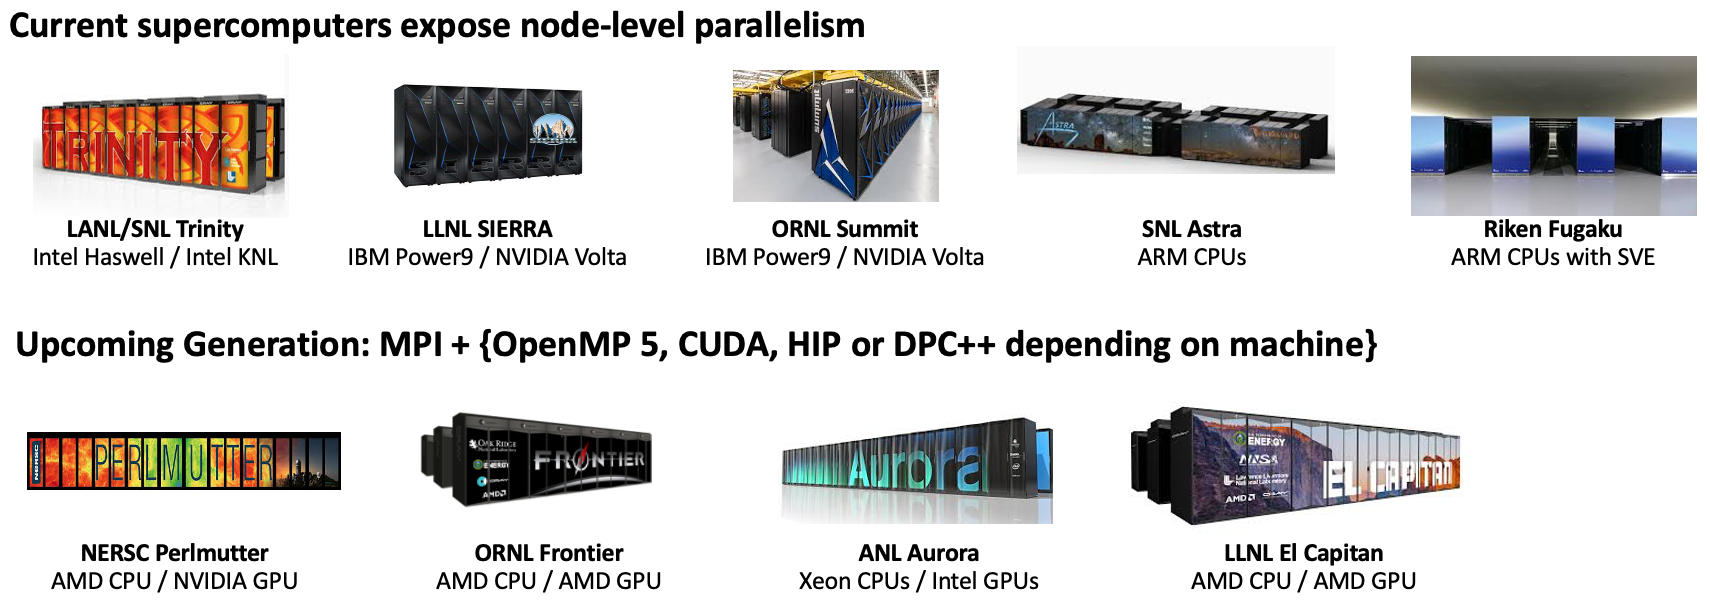
\includegraphics[width=1.05\textwidth]{figures/Architecture-Overview-MPI}
  \end{center}

\begin{itemize}
	\item Today supercomputers are clusters with disjoint address spaces
	\item One additional level of concurrency: node-level
	\item Allow MPI+Kokkos hybrid applications (using patterns, views, spaces, etc.)
\end{itemize}

\end{frame}

\begin{frame}[fragile]{MPI + Kokkos}
\textbf{Why mix MPI with Kokkos}
\begin{itemize}
  \item Need to address internode data transfers
  \item MPI is the de-facto standard
  \item MPI is well supported on all platforms
  \begin{itemize}
     \item MPI also knows how to talk to GPUs
  \end{itemize}
  \item The legacy code you want to port is already using MPI
  \item Programming explicitly to the parallelism hierarchy can help
\end{itemize}

\pause
\textbf{Are there any alternatives?}
\begin{itemize}
  \item You can potentially use PGAS models (discussed later).
  \item Global tasking models may work for you
  \begin{itemize}
    \item Kokkos has been used with Uintah for years
    \item LANL explores combining Legion and Kokkos with our support
  \end{itemize}
\end{itemize}
\end{frame}

\begin{frame}[fragile]{Motivating Example - Vector Shift}
  Simple Shifting of data:

  \begin{code}[keywords={View,double,int}]
  View<double*> A("A",N), B("B",N);
  // Single Device
  parallel_for("Shift",N,KOKKOS_LAMBDA(int i) {
    B((i+K)%N) = A(i);
  });
  \end{code}

\pause
  Lets assume we have R ranks:
  \begin{itemize}
    \item Now each rank owns N/R elements
    \item Rank j needs to send K elements to rank j+1
      \begin{itemize}
         \item j is sending the last K elements of A
      \end{itemize}
    \item Rank j needs to receive K elements from rank j-1
      \begin{itemize}
         \item j is receiving into the first K elements of B
      \end{itemize}
  \end{itemize}
\end{frame}

\begin{frame}[fragile]{Hybrid Programming 1}
\begin{itemize}
 \item The MPI Interface uses raw pointers
 \begin{lstlisting}
Kokkos::View<...> recv_view(...);
Kokkos::View<...> send_view(...);
void* recv_ptr = recv_view.data();
void* send_ptr = send_view.data();
  \end{lstlisting}
 \item Data needs to be stored contiguously $\Rightarrow$ \texttt{LayoutStride} not possible
 \item Data stored on the device requires GPU-aware MPI implementations. Otherwise, copying to the host is necessary
 \begin{lstlisting}
auto recv_view_h = Kokkos::create_mirror_view_and_copy(
  Kokkos::DefaultHostExecutionSpace{}, recv_view_d);
auto send_view_h = Kokkos::create_mirror_view_and_copy(
  Kokkos::DefaultHostExecutionSpace{}, send_view_d);
void* recv_ptr = recv_view_h.data();
void* send_ptr = send_view_h.data();
  \end{lstlisting}
\end{itemize}
\end{frame}

\begin{frame}[fragile]{Hybrid Programming 1}
Then the usual MPI functions can be used:

\vspace{10pt}
 \begin{code}[keywords={MPI_Request,MPI_Irecv,MPI_Isend,MPI_Waitall}]
MPI_Request requests[2];
MPI_Irecv(recv_ptr,recv_view.size(),MPI_DOUBLE,
          source,1,MPI_COMM_WORLD,&requests[0]);
// Send the buffer
MPI_Isend(send_ptr,send_view.size(),MPI_DOUBLE,
          target,1,MPI_COMM_WORLD,&requests[1]);
// Wait for communication to finish
MPI_Waitall(2,requests,MPI_STATUSES_IGNORE);
  \end{code}

\pause
\vspace{10pt}
In our example \texttt{send\_view} and \texttt{recv\_view} are just subviews:

\vspace{5pt}
\begin{code}[keywords={subview,make_pair,auto}]
auto send_view = Kokkos::subview(A,std::make_pair(myN-K, myN));
auto recv_view = Kokkos::subview(B,std::make_pair(0, K));
\end{code}
\end{frame}

\begin{frame}[fragile]{Simple Overlapping Communication}
  \textbf{Overlap communication with computation if possible!}

  \begin{itemize}
     \item Make sure compute kernel don not access send/recv buffers
     \item Post sends and recvs first
     \item Launch kernel
     \item Wait on MPI
  \end{itemize}

  \pause
  Vector-Shift Example:
\begin{code}[keywords={subview,MPI_Request,MPI_Irecv,MPI_Isend,parallel_for,MPI_Waitall}]
auto send_view = Kokkos::subview(A,std::make_pair(myN-K, myN));
auto recv_view = Kokkos::subview(B,std::make_pair(0, K));
MPI_Request requests[2];
// Post sends/recv
MPI_Irecv(recv_ptr,recv_view.size(),MPI_DOUBLE,
          source,1,MPI_COMM_WORLD,&requests[0]);
MPI_Isend(send_ptr,send_view.size(),MPI_DOUBLE,
          target,1,MPI_COMM_WORLD,&requests[1]);
parallel_for("ShiftA",RangePolicy<>(K,myN), 
  KOKKOS_LAMBDA(int i) { B(i) = A(i-K); });
// Wait for communication to finish
MPI_Waitall(2,requests,MPI_STATUSES_IGNORE);
\end{code}
\end{frame}


\begin{frame}[fragile]{Initializing MPI}
\textbf{Technical requirements}
\begin{itemize}
    \item Initialize MPI before Kokkos
    \begin{lstlisting}
int main(int argc, char* argv[]) {
  MPI_Init(&argc,&argv);
  Kokkos::initialize(argc,argv);
  [...]
  Kokkos::finalize();
  MPI_Finalize();
  }
    \end{lstlisting}
    \item By default, GPUs are distributed in a round-robin fashion if there are multiple.
	\item Use \texttt{mpicxx} as compiler
 	and \texttt{OMPI\_CXX=<path-to-kokkos-install>/nvcc\_wrapper} (for OpenMPI)
  	or use
\begin{texttt}find\_package(MPI REQUIRED)\end{texttt}
 with \texttt{CMake}.
\end{itemize}
\end{frame}


\begin{frame}[fragile]{Exercise: Send Data between MPI Processes}

  \begin{small}
  \begin{itemize}
  \item Location: \ExerciseDirectory{mpi\_pack\_unpack}
  \item Add missing MPI calls to \texttt{RunPackCommUnpackTest::run\_comm()}.
  \item Compile and run on CPU, and then on GPU.
  \end{itemize}
  \end{small}

\begin{code}
mkdir build && cd build
export Kokkos_DIR=<path-to-kokkos-install>
cmake .. && make
# Run exercise
mpiexec -np 2 MPIPackUnpack
\end{code}

Command line arguments
%   \begin{scriptsize}
  \begin{itemize}
  \item Vary size of data
  \item Vary size of buffers
  \item Number of repeats for timing
  \item Copy to host first
  \end{itemize}
%   \end{scriptsize}
\end{frame}

\begin{frame}[fragile]{Explicit Message Buffers}
\textbf{Sometimes extra send/recv buffers are needed}
\begin{itemize}
  \item Buffer data which is getting written to again
  \item Sparse data needs to be sent or received
    \begin{itemize}
       \item In particular if isn't regular strided
       \item Will discuss some best practices later
    \end{itemize}
  \item The system doesn't allow MPI to access some memory space
\end{itemize}

\pause
\textbf{The Pack-Send/Recv-Unpack Cycle:}
\begin{itemize}
  \item Post Irecvs
  \item Pack buffers
  \item Post Isends
  \item Wait on message completion
  \item Unpack buffers
\end{itemize}
\end{frame}

\begin{frame}[fragile]{Explicit Message Buffers}
Based on our Kokkos knowledge of Execution and Memory Spaces the following question arises:

\textbf{Where should the pack kernel run, and where should it pack to?}

\begin{itemize}
  \item Run the pack kernel wherever the data lives.
  \item The best memory space for the pack buffer depends.
  \item Sometimes packing into a device buffer, and still explicitly copying to the host is best.
\end{itemize}

\textit{There are a number of options for CUDA for example:}

\vspace{5pt}
\begin{tabular}{l|l|l}
\textbf{Data Space} & \textbf{Pack Buffer Space} & \textbf{Explicit HostCopy} \\ \hline
CudaSpace & CudaSpace & yes \\
CudaSpace & CudaSpace & no \\
CudaSpace & CudaUVMSpace & no \\
CudaSpace & CudaHostPinnedSpace & no \\
\end{tabular}

\end{frame}

\begin{frame}[fragile]{Performance Results}

\textbf{CudaSpace vs CudaUVMSpace vs CudaHostPinnedSpace}
\begin{itemize}
\item Time relative to CudaSpace on single socket (lower is better).
\item Performance is very sensitive to system and configurations!!
\end{itemize}

\pause
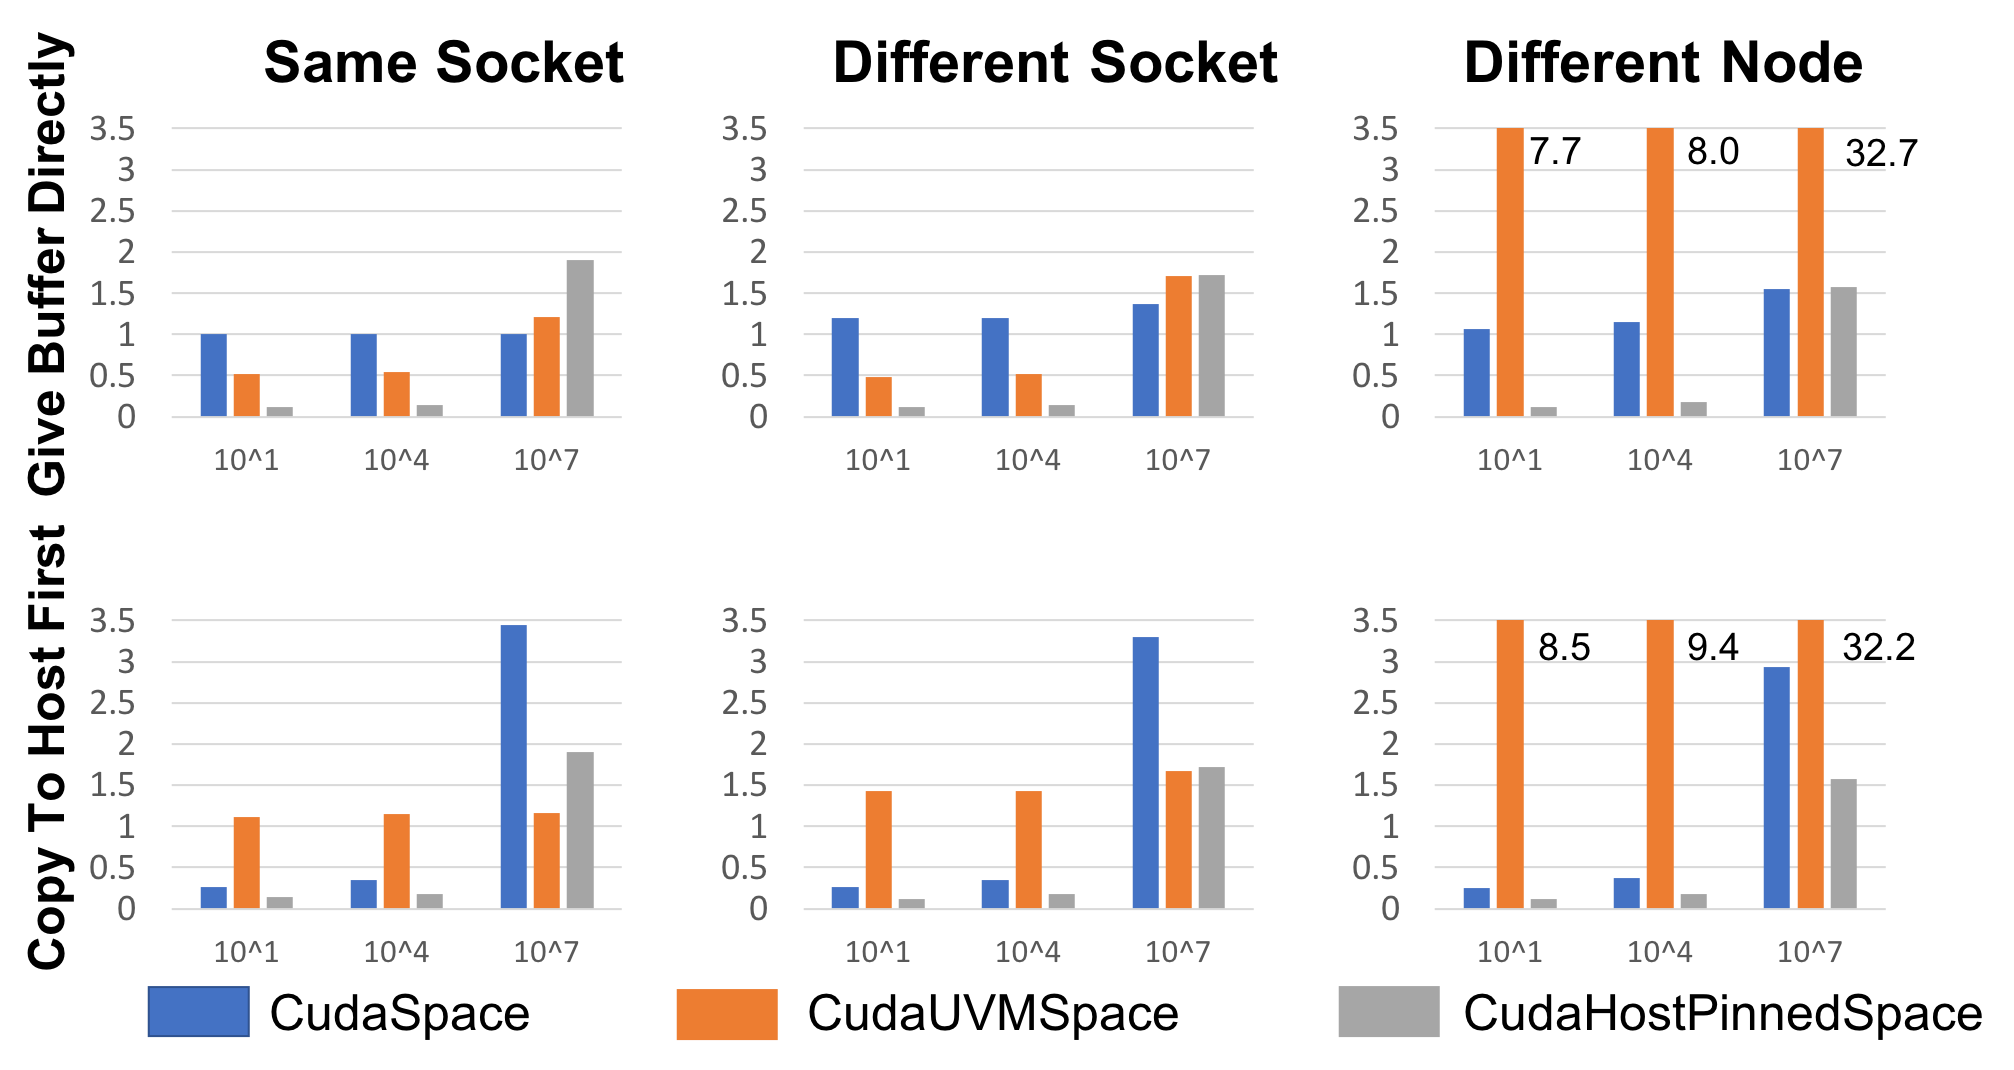
\includegraphics[width=\textwidth]{figures/MPI-Performance}
\end{frame}

\begin{comment}
\begin{frame}[fragile]{Performance Results Exercise}
Excluding parallel\_fors, copy to host
     \pgfplotstableread{
 size      Cuda       CudaHostPinnedh CudaUVM   Host
 10        0.0000533  0.0000171       0.0003804 0.0000178
 100       0.0000541  0.0000174       0.0003738 0.0000178
 1000      0.0000584  0.0000180       0.0003736 0.0000191
 10000     0.0000797  0.0000228       0.0003794 0.0000238
 100000    0.0002245  0.0000468       0.0003948 0.0000478
 1000000   0.0020995  0.0005860       0.0006549 0.0005916
 10000000  0.0191008  0.0065910       0.0035631 0.0066248
 100000000 0.1940944  0.0663647       0.0347974 0.0656929
}\tablecompareperformance

\begin{figure}
\centering
\begin{tikzpicture}[scale=0.9]
    \begin{loglogaxis}[
      legend style={legend pos=north west},
      xlabel={N},
      ylabel={time in (s)},
      ymin=1e-5,
      ymax=1,
      grid, thick
    ]
      \addplot table[x expr={\thisrowno{0}}, y index={1}] {\tablecompareperformance};
      \addlegendentry{Cuda}
      \addplot table[x expr={\thisrowno{0}}, y index={2}] {\tablecompareperformance};
      \addlegendentry{CudaHostPinned}
      \addplot table[x expr={\thisrowno{0}}, y index={3}] {\tablecompareperformance};
      \addlegendentry{CudaUVM}
      \addplot table[x expr={\thisrowno{0}}, y index={4}] {\tablecompareperformance};
      \addlegendentry{Host}
      \end{loglogaxis}
    \end{tikzpicture}
\end{figure}
\end{frame}

\begin{frame}[fragile]{Performance Results Exercise}
Excluding parallel\_fors, don't copy to host
     \pgfplotstableread{
 size      Cuda       CudaHostPinnedh CudaUVM   Host
 10        0.00033222 0.00001230      0.00011110 0.00001225
 100       0.00033221 0.00001281      0.00011025 0.00001258
 1000      0.00033359 0.00001356      0.00011182 0.00001417
 10000     0.00033872 0.00001800      0.00011358 0.00001819
 100000    0.00035633 0.00004147      0.00013237 0.00004257
 1000000   0.00053719 0.00053546      0.00042869 0.00051637
 10000000  0.00216941 0.00659140      0.00388138 0.00657494
 100000000 0.01844423 0.06551141      0.03870359 0.06524309
}\tablecompareperformancegpuaware

\begin{figure}
\centering
\begin{tikzpicture}[scale=0.9]
    \begin{loglogaxis}[
      legend style={legend pos=north west},
      xlabel={N},
      ylabel={time in (s)},
      ymin=1e-5,
      ymax=1,
      grid, thick
    ]
      \addplot table[x expr={\thisrowno{0}}, y index={1}] {\tablecompareperformancegpuaware};
      \addlegendentry{Cuda}
      \addplot table[x expr={\thisrowno{0}}, y index={2}] {\tablecompareperformancegpuaware};
      \addlegendentry{CudaHostPinned}
      \addplot table[x expr={\thisrowno{0}}, y index={3}] {\tablecompareperformancegpuaware};
      \addlegendentry{CudaUVM}
      \addplot table[x expr={\thisrowno{0}}, y index={4}] {\tablecompareperformancegpuaware};
      \addlegendentry{Host}
      \end{loglogaxis}
    \end{tikzpicture}
\end{figure}
\end{frame}

\begin{frame}[fragile]{Performance Results Exercise}
different sockets
     \pgfplotstableread{
 size      Cuda       CudaHostPinnedh CudaUVM    Host
 10        0.041782   0.003966        0.017534   0.001408
 10000     0.041473   0.005486        0.018058   0.027909
 10000000  1.232990   1.551578        1.534636   72.761595
}\tablecompareperformancefull

\begin{figure}
\centering
\begin{tikzpicture}[scale=0.9]
    \begin{loglogaxis}[
      legend style={legend pos=north west},
      xlabel={N},
      ylabel={time in (s)},
      ymin=1e-3,
      ymax=100,
      grid, thick
    ]
      \addplot table[x expr={\thisrowno{0}}, y index={1}] {\tablecompareperformancefull};
      \addlegendentry{Cuda}
      \addplot table[x expr={\thisrowno{0}}, y index={2}] {\tablecompareperformancefull};
      \addlegendentry{CudaHostPinned}
      \addplot table[x expr={\thisrowno{0}}, y index={3}] {\tablecompareperformancefull};
      \addlegendentry{CudaUVM}
      \addplot table[x expr={\thisrowno{0}}, y index={4}] {\tablecompareperformancefull};
      \addlegendentry{Host}
      \end{loglogaxis}
    \end{tikzpicture}
\end{figure}
\end{frame}

\begin{frame}[fragile]{Performance Results Exercise}
different sockets, copy to host
     \pgfplotstableread{
 size      Cuda       CudaHostPinnedh CudaUVM    Host
 10        0.008601   0.004460        0.046049   0.001922
 10000     0.012437   0.005989        0.049750   0.028535
 10000000  2.969337   1.551063        1.505497   71.818246
}\tablecompareperformancefullhost

\begin{figure}
\centering
\begin{tikzpicture}[scale=0.9]
    \begin{loglogaxis}[
      legend style={legend pos=north west},
      xlabel={N},
      ylabel={time in (s)},
      ymin=1e-3,
      ymax=100,
      grid, thick
    ]
      \addplot table[x expr={\thisrowno{0}}, y index={1}] {\tablecompareperformancefullhost};
      \addlegendentry{Cuda}
      \addplot table[x expr={\thisrowno{0}}, y index={2}] {\tablecompareperformancefullhost};
      \addlegendentry{CudaHostPinned}
      \addplot table[x expr={\thisrowno{0}}, y index={3}] {\tablecompareperformancefullhost};
      \addlegendentry{CudaUVM}
      \addplot table[x expr={\thisrowno{0}}, y index={4}] {\tablecompareperformancefullhost};
      \addlegendentry{Host}
      \end{loglogaxis}
    \end{tikzpicture}
\end{figure}
\end{frame}

\begin{frame}[fragile]{Performance Results Exercise}
same sockets
     \pgfplotstableread{
 size      Cuda       CudaHostPinnedh CudaUVM    Host
 10        0.035284   0.004108        0.018218   0.001452
 10000     0.035542   0.005595        0.018763   0.033356
 10000000  0.900193   1.708386        1.087862   87.032740
}\tablecompareperformancefullsocket

\begin{figure}
\centering
\begin{tikzpicture}[scale=0.9]
    \begin{loglogaxis}[
      legend style={legend pos=north west},
      xlabel={N},
      ylabel={time in (s)},
      ymin=1e-3,
      ymax=100,
      grid, thick
    ]
      \addplot table[x expr={\thisrowno{0}}, y index={1}] {\tablecompareperformancefullsocket};
      \addlegendentry{Cuda}
      \addplot table[x expr={\thisrowno{0}}, y index={2}] {\tablecompareperformancefullsocket};
      \addlegendentry{CudaHostPinned}
      \addplot table[x expr={\thisrowno{0}}, y index={3}] {\tablecompareperformancefullsocket};
      \addlegendentry{CudaUVM}
      \addplot table[x expr={\thisrowno{0}}, y index={4}] {\tablecompareperformancefullsocket};
      \addlegendentry{Host}
      \end{loglogaxis}
    \end{tikzpicture}
\end{figure}
\end{frame}

\begin{frame}[fragile]{Performance Results Exercise}
same sockets, copy to host
     \pgfplotstableread{
 size      Cuda       CudaHostPinnedh CudaUVM    Host
 10        0.009128   0.004699        0.039293   0.002084
 10000     0.012310   0.006289        0.040151   0.028537
 10000000  3.799518   1.708801        1.036396   85.849318
}\tablecompareperformancefullhostsocket

\begin{figure}
\centering
\begin{tikzpicture}[scale=0.9]
    \begin{loglogaxis}[
      legend style={legend pos=north west},
      xlabel={N},
      ylabel={time in (s)},
      ymin=1e-3,
      ymax=100,
      grid, thick
    ]
      \addplot table[x expr={\thisrowno{0}}, y index={1}] {\tablecompareperformancefullhostsocket};
      \addlegendentry{Cuda}
      \addplot table[x expr={\thisrowno{0}}, y index={2}] {\tablecompareperformancefullhostsocket};
      \addlegendentry{CudaHostPinned}
      \addplot table[x expr={\thisrowno{0}}, y index={3}] {\tablecompareperformancefullhostsocket};
      \addlegendentry{CudaUVM}
      \addplot table[x expr={\thisrowno{0}}, y index={4}] {\tablecompareperformancefullhostsocket};
      \addlegendentry{Host}
      \end{loglogaxis}
    \end{tikzpicture}
\end{figure}
\end{frame}

\begin{frame}[fragile]{Performance Results Exercise}
different node
     \pgfplotstableread{
 size      Cuda       CudaHostPinnedh CudaUVM    Host
 10        0.036866   0.003910        0.270404   0.001427
 10000     0.039647   0.006262        0.283026   0.029009
 10000000  1.396050   1.415000        29.371574  73.402895
}\tablecompareperformancefullnode

\begin{figure}
\centering
\begin{tikzpicture}[scale=0.9]
    \begin{loglogaxis}[
      legend style={legend pos=north west},
      xlabel={N},
      ylabel={time in (s)},
      ymin=1e-3,
      ymax=100,
      grid, thick
    ]
      \addplot table[x expr={\thisrowno{0}}, y index={1}] {\tablecompareperformancefullnode};
      \addlegendentry{Cuda}
      \addplot table[x expr={\thisrowno{0}}, y index={2}] {\tablecompareperformancefullnode};
      \addlegendentry{CudaHostPinned}
      \addplot table[x expr={\thisrowno{0}}, y index={3}] {\tablecompareperformancefullnode};
      \addlegendentry{CudaUVM}
      \addplot table[x expr={\thisrowno{0}}, y index={4}] {\tablecompareperformancefullnode};
      \addlegendentry{Host}
      \end{loglogaxis}
    \end{tikzpicture}
\end{figure}
\end{frame}

\begin{frame}[fragile]{Performance Results Exercise}
different node, copy to host
     \pgfplotstableread{
 size      Cuda       CudaHostPinnedh CudaUVM    Host
 10        0.008674   0.004455        0.298826   0.001864
 10000     0.013019   0.006524        0.330559   0.040083
 10000000  2.640824   1.422987        29.231414  73.752908
}\tablecompareperformancefullhostnode

\begin{figure}
\centering
\begin{tikzpicture}[scale=0.9]
    \begin{loglogaxis}[
      legend style={legend pos=north west},
      xlabel={N},
      ylabel={time in (s)},
      ymin=1e-3,
      ymax=100,
      grid, thick
    ]
      \addplot table[x expr={\thisrowno{0}}, y index={1}] {\tablecompareperformancefullhostnode};
      \addlegendentry{Cuda}
      \addplot table[x expr={\thisrowno{0}}, y index={2}] {\tablecompareperformancefullhostnode};
      \addlegendentry{CudaHostPinned}
      \addplot table[x expr={\thisrowno{0}}, y index={3}] {\tablecompareperformancefullhostnode};
      \addlegendentry{CudaUVM}
      \addplot table[x expr={\thisrowno{0}}, y index={4}] {\tablecompareperformancefullhostnode};
      \addlegendentry{Host}
      \end{loglogaxis}
    \end{tikzpicture}
\end{figure}
\end{frame}
\end{comment}

\begin{frame}[fragile]{Explicit Message Buffers}
\textbf{Leveraging streams allow calculations and communication with explicit buffers to overlap!}
\begin{itemize}
  \item Execute packing, unpacking and deep\_copies with different streams than interior kernels.
  \item Submission order is important though
  \begin{itemize}
     \item Worksets are largely worked on in submission order even with CUDA streams
     \item Need to submit pack kernels first, then interiors kernel
     \item Unless priority streams are a thing ...
  \end{itemize}
  \item Fence the pack execution space instances only before issuing sends
  \item ExecutionSpace instances, and buffers need to be persistent - allocations add fencing
\end{itemize}
\end{frame}

\begin{frame}[fragile]{Explicit Message Buffers}
\textbf{Code Skeleton:}
\begin{code}[keywords={MPI_Irecv,parallel_for,fence,MPI_Isend,MPI_Waitall}]
  // Create execution space instances
  ExecSpace exec_pack(..), exec_comp(..);
  using exec_policy = RangePolicy<ExecSpace>;
  // Post Receives
  MPI_Irecv(...);
  // Launch pack kernel in pack exec instance
  // Likely this uses only few cores
  parallel_for("PackBuffer",
    exec_policy(exec_pack,0,N),fpack);
  // Launch compute kernel independent of message exchange
  parallel_for("Interior",
    exec_policy(exec_comp,0,N),finterior);
  // Wait for pack kernel to finish before sending data
  exec_pack.fence();
  MPI_Isend(...);
  // Wait for communication to finish
  MPI_Waitall(...);
  // Unpack received data - may still overlap with "Interior"
  parallel_for("UnpackBuffer",
    exec_policy(exec_pack,0,N),funpack);
  // Wait for all work to finish
  Kokkos::fence();
\end{code}

\end{frame}

\begin{frame}{Motivating Example - Heat Equation}
\textbf{3D Heat Conduction}
\begin{itemize}
\item Heat conduction inside the body
\item Thermal radiation (Black Body) on surface
\item Incoming power flow from one direction
\end{itemize}

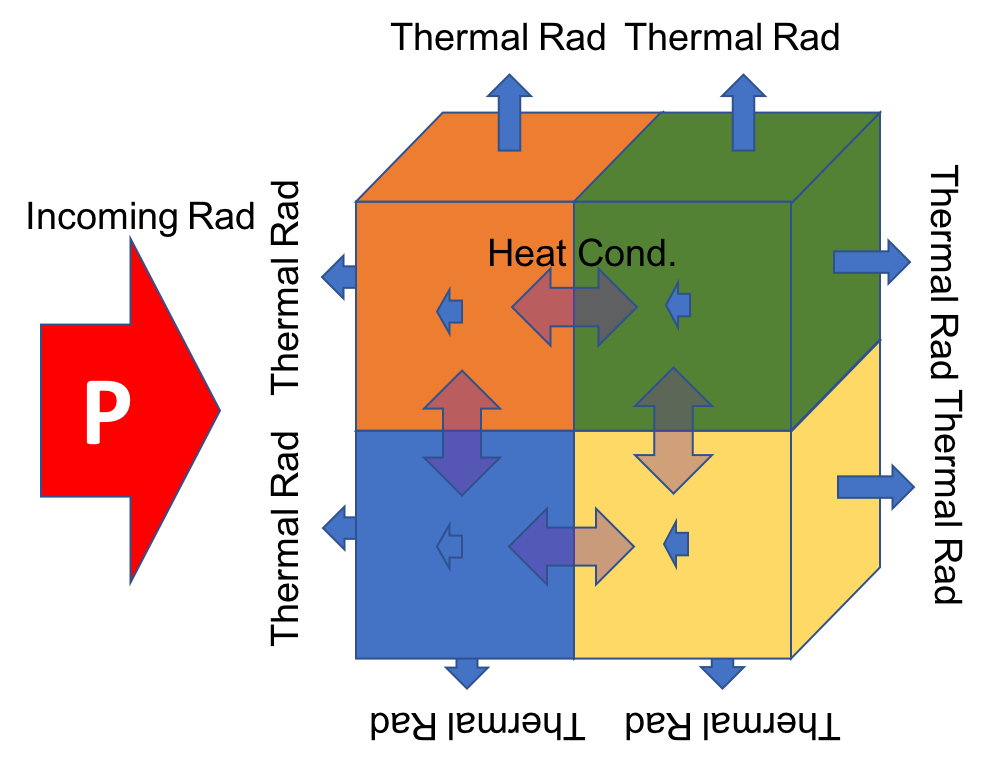
\includegraphics[width=0.65\textwidth]{figures/3DHeat}
\end{frame}

\begin{comment}
\begin{frame}{Motivating Example - Heat Equation}
Models distribution of heat given a heat source/sink $f$ over time
    \begin{align*}
       \partial_t u - \alpha \Delta_x u = f
    \end{align*}
    Using explicit Euler for time discretization gives
    \begin{align*}
       u^{n+1} = u^n + \Delta t (\alpha \Delta_x u^n + f(t_n))
    \end{align*}
    Finite difference discretization using central differences
    \begin{align*}
          u_{ijk}^{n+1} =& u_{ijk}^n + \Delta t f(t_n) \\
                         &+\frac{\Delta t}{h^2}\alpha (u_{i-1,j,k}^n -2 u_{i,j,k}^n + u_{i+1,j,k}^n \\
                         &\qquad\qquad+ u_{i,j-1,k}^n -2 u_{i,j,k}^n + u_{i,j+1,k}^n \\
                         &\qquad\qquad+ u_{i,j,k-1}^n -2 u_{i,j,k}^n + u_{i,j,k+1}^n)
    \end{align*}
\end{frame}

\begin{frame}{Motivating Example - Heat Equation}
Discretization
    \begin{align*}
          u_{ijk}^{n+1} =& u_{ijk}^n + \Delta t f(t_n) \\
                         &+\frac{\Delta t}{h^2}\alpha (u_{i-1,j,k}^n -2 u_{i,j,k}^n + u_{i+1,j,k}^n \\
                         &\qquad\qquad+ u_{i,j-1,k}^n -2 u_{i,j,k}^n + u_{i,j+1,k}^n \\
                         &\qquad\qquad+ u_{i,j,k-1}^n -2 u_{i,j,k}^n + u_{i,j,k+1}^n)
    \end{align*}
    \begin{itemize}
    \item Updating $u_{ijk}$ requires information for all the (direct) neighbors.
    \item Splitting the computational domain across multiple processes requires exchange of data $\Rightarrow$ MPI
    \end{itemize}

\end{frame}

\begin{frame}{Example - 3D Heat Equations}
  \textbf{Heat Source / Sink defined through the boundary conditions}
   \begin{itemize}
      \item Using surface black body thermal radiation as heat sink
      \begin{itemize}
        \item Using A as surface area of an element (its zero for all bulk elements)
      \end{itemize}
      \item Using a constant power density as heat source on one surface
      \begin{itemize}
        \item Turn the power of mid run.
        \item Use Ax as surface area exposed to the heat source
      \end{itemize}
   \end{itemize}
   \begin{align*}
      f(t_n) = -A_{ijk}*sigma*u^4 + Ax_{ijk}*P(t_n)
   \end{align*}
\end{frame}
\end{comment}

\begin{frame}{Simple Approach}
   \textbf{No Overlapping}

Data Structures:
\begin{itemize}
  \item T(x,y,z): temperature in cell (x,y,z)
  \item dT(x,y,z): temperature change in time increment dt
  \item T\_{left,right,up,down,front,back}: recv buffers for boundaries
  \item T\_{left\_out,...}: send buffers for boundaries
\end{itemize}

Time approach:
\begin{itemize}
  \item deep\_copy boundary layers as needed to contiguous send buffers
  \item Post MPI send/recv with send/recv buffers
  \item Launch kernel for interior elements doing heat conduction only
  \item Wait for MPI
  \item Compute updates for boundary elements using the recv buffers
\end{itemize}
\end{frame}

\begin{frame}{Optimized Pattern}
\textbf{Overlapping packing/unpacking with interior compute}

Getting better performance can be achieved by staging calls correctly, and using execution space instances:

\begin{itemize}
  \item Use 7 instances: interior, 6x boundary (left, right, ...)
  \item Issue Irecv
  \item Run up to 6 pack kernels using different exec space instances
  \item Launch interior kernel into its own instance
  \item Fence first boundary pack instance, issue Isend
  \item Fence other boundary packs and issue Isends one by one
  \item Wait for MPI operations to finish
  \item Issue boundary temperature update kernel
  \item Fence everything
\end{itemize}
\end{frame}

\begin{frame}[fragile]{Exercise: Optimize 3D Heat}
Optimize the basic MPI implementation of the 3D heat conduction code for GPU systems.

  \vspace{10pt}

  \textbf{Details}:
  \begin{small}
  \begin{itemize}
\item Location: \ExerciseDirectory{mpi\_heat\_conduction}
\item Use Execution Space instances for more overlapping
\item Order operations for maximum overlapping
\item Run with correct GPU mapping
\end{itemize}
  \end{small}

\ul{\textbf{Things to try:}}
  \begin{small}
  \begin{itemize}
  \item Try strong vs weak scaling
  \item Change Problem Size -X , -Y , -Z
  \item Play with buffer memory space
  \item Compare same socket, vs different socket, vs multi node perf
  \end{itemize}
  \end{small}
\end{frame}

\begin{frame}[fragile]{Sparse Data to be Send}
In the heat conduction example some surfaces were sparse, but regular.

\pause
\vspace{10pt}
\textbf{How best to generate index lists if data is not regular sparse?}

\pause
\vspace{10pt}
Example problems:
\begin{itemize}
  \item Send all particles which crossed the boundary.
  \item Send all elements in contact with the surface.
\end{itemize}

\pause
Use indirect pack kernel:
\begin{code}[keywords={parallel_for,send_list}]
  parallel_for("Pack",num_send, KOKKOS_LAMBDA(int e) {
    pack(e) = data(send_list(e));
  });
\end{code}

\pause
\textbf{How to generate the send\_list?}

\pause
$=>$ Use a \texttt{parallel\_scan}

\end{frame}


\begin{frame}[fragile]{Generating Index}

\textbf{Generating Index Lists via \texttt{parallel\_scan}}

\vspace{10pt}
\begin{itemize}
  \item \texttt{bool needs\_send(int e)} is true if element \texttt{e} needs to be sent:
\end{itemize}

\begin{code}[keywords={parallel_scan,send_list,final}]
parallel_scan("GenIDX",num_elements,
  KOKKOS_LAMBDA(int e, int& idx, bool final){
  if(needs_send(e)) {
    if(final) send_list(idx) = e;
    idx++;
  }
});
\end{code}

\pause
\vspace{10pt}
\textbf{What if you don't know how large send\_list needs to be?}

$=>$ Use parallel\_scan with return argument; Repeat if count exceeds size.
\end{frame}

\begin{frame}[fragile]{Generating Index Lists}
\textbf{Merged Count - Allocate - Fill pattern}
\begin{code}[keywords={parallel_scan,count,send_list,needs_send}]
// Initial Count Guess
int count = K;
send_list.resize(count);
parallel_scan("GenIDX1",N,KOKKOS_LAMBDA(int e, int& idx, bool f) {
  if(needs_send(e)) {
    // Only add if its smaller but keep counting
    if(final && idx<count) { send_list(idx)=e; } idx++;
  }
},count);
// If count indicates you ran over redo the kernel
if(count>send_list.extent(0)) {
  send_list.resize(count);
  parallel_scan("GenIDX2",N,KOKKOS_LAMBDA(int e, int& idx, bool f) {
    if(needs_send(e)) { if(final) { send_list(idx)=e; } idx++; }
  },count);
}
\end{code}

\vspace{-5pt}
\begin{itemize}
  \item Worst case scenario: 2x cost
  \item If you remember count you will reach often steady state
  \item More complex memory pool based algorithms are often costly
\end{itemize}
\end{frame}


\begin{frame}{Resource Affinity}
\textbf{CPU Core Assignment:}
\begin{itemize}
  \item Don't oversubscribe your CPU cores!
  \item By default for example each rank will use all cores in OpenMP
  \item Set process masks appropriately
  \begin{itemize}
    \item OpenMPI: mpirun -np R --map-by socket=PE:4
    \item mpich:
    \item SLURM:
  \end{itemize}
\end{itemize}

\vspace{10pt}
\textbf{GPU Assignment:}
\begin{itemize}
	\item By default, Kokkos will assign GPUs round robin i.e. MPI\_Rank\%num\_visible\_devices
	\item If you need to mask out some GPUs on a node
        \begin{itemize}
           \item env variable KOKKOS\_VISIBLE\_DEVICES="0,3"
        \end{itemize}
\end{itemize}
\textbf{Note:} \texttt{jsrun} on \texttt{Summit} needs \texttt{--smpiargs="-gpu"} for GPU-aware MPI communication.
\end{frame}



\begin{frame}{Summary}
\textbf{Simple MPI and Kokkos Interaction is easy!}
\begin{itemize}
  \item Simply pass \texttt{data()} of a View to MPI functions plus its size.
  \begin{itemize}
    \item But it better be a contiguous View!
  \end{itemize}
  \item Initialize Kokkos after MPI, and finalize it before MPI
\end{itemize}

\vspace{10pt}
\textbf{Overlapping communication and computation possible}
\begin{itemize}
  \item Use Execution Space instances to overlap packing/unpacking with other computation.
  \item Order operations to maximize overlapping potential. 
\end{itemize}
\end{frame}

%=============================================
%=============================================
%=============================================

\begin{frame}[fragile]

  {\Huge Kokkos Remote Spaces: Support for PGAS in Kokkos}

  \vspace{10pt}

  {\large How to write a PGAS application with Kokkos.}

  \vspace{20pt}

  \textbf{Learning objectives:}
  \begin{itemize}
    \item {How to create global Views.}
    \item {How access global data.}
    \item {Taking a closer look at SPMV (CG).}
  \end{itemize}

  \vspace{-20pt}

\end{frame}


%=============================================
%=============================================
%=============================================

\begin{frame}[fragile]{Remote Spaces: Motivation}
  \textbf{Previous Example: \texttt{Vector-Shift}}
  \vspace{12pt}
  \center
  \begin{center}
  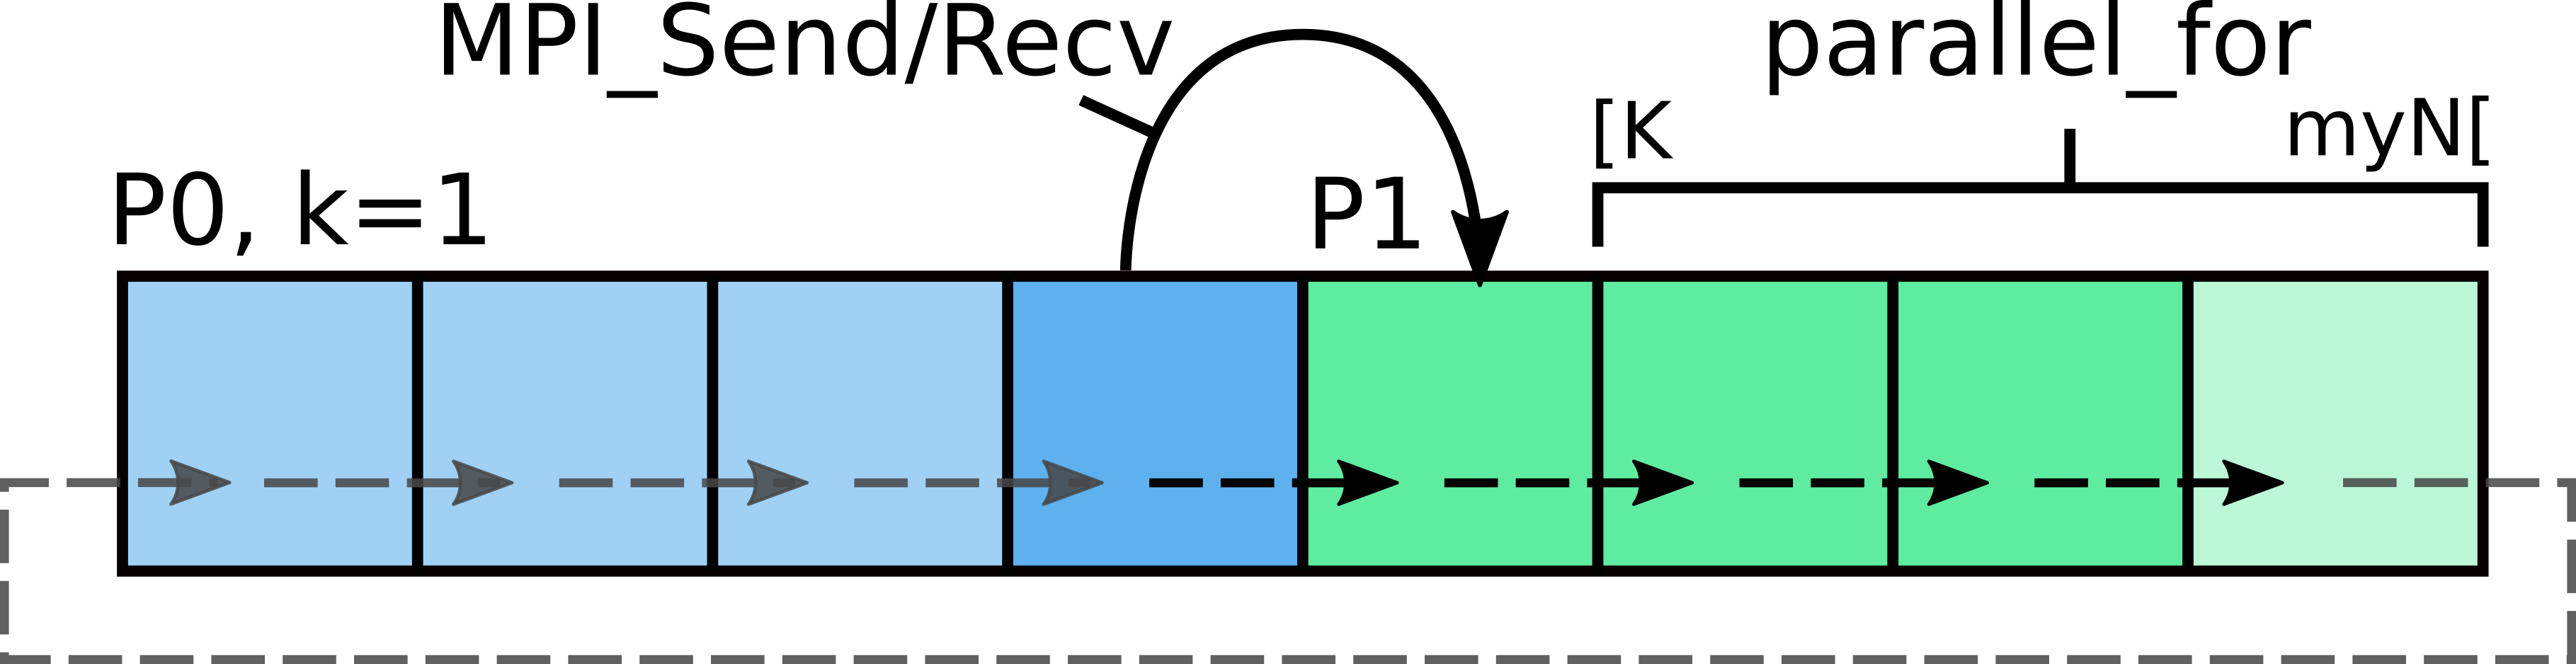
\includegraphics[width=0.50\textwidth]{figures/VectorShift}
  \end{center}
  \begin{code}[keywords={recv_ptr, send_ptr, send_view, recv_view,double,
  KOKKOS_LAMBDA,MPI_Irecv,MPI_Isend,parallel_for, MPI_Waitall}]
  auto send_view = Kokkos::subview(A,std::make_pair(myN-K, myN));
  auto recv_view = Kokkos::subview(B,std::make_pair(0, K));
  ...
  MPI_Request requests[2];
  MPI_Irecv(recv_ptr,recv_view.size(),MPI_DOUBLE,
            source,1,MPI_COMM_WORLD,&requests[0]);
  MPI_Isend(send_ptr,send_view.size(),MPI_DOUBLE,
            target,1,MPI_COMM_WORLD,&requests[1]);
  parallel_for("Shift",RangePolicy<>(K,myN), 
    KOKKOS_LAMBDA(int i) { B(i) = A(i-K); });
  MPI_Waitall(2,requests,MPI_STATUSES_IGNORE);
  \end{code}
  \begin{itemize}
    \item \textbf{How to simplify communication, and reduce host-device data movement?}
    \end{itemize}
\end{frame}

%=============================================
%=============================================
%=============================================

\begin{frame}[fragile]{Remote Spaces: The PGAS Model}
  \vspace{15pt}
  \textbf{PGAS (Partitioned Global Address Space)}
  \begin{center}
    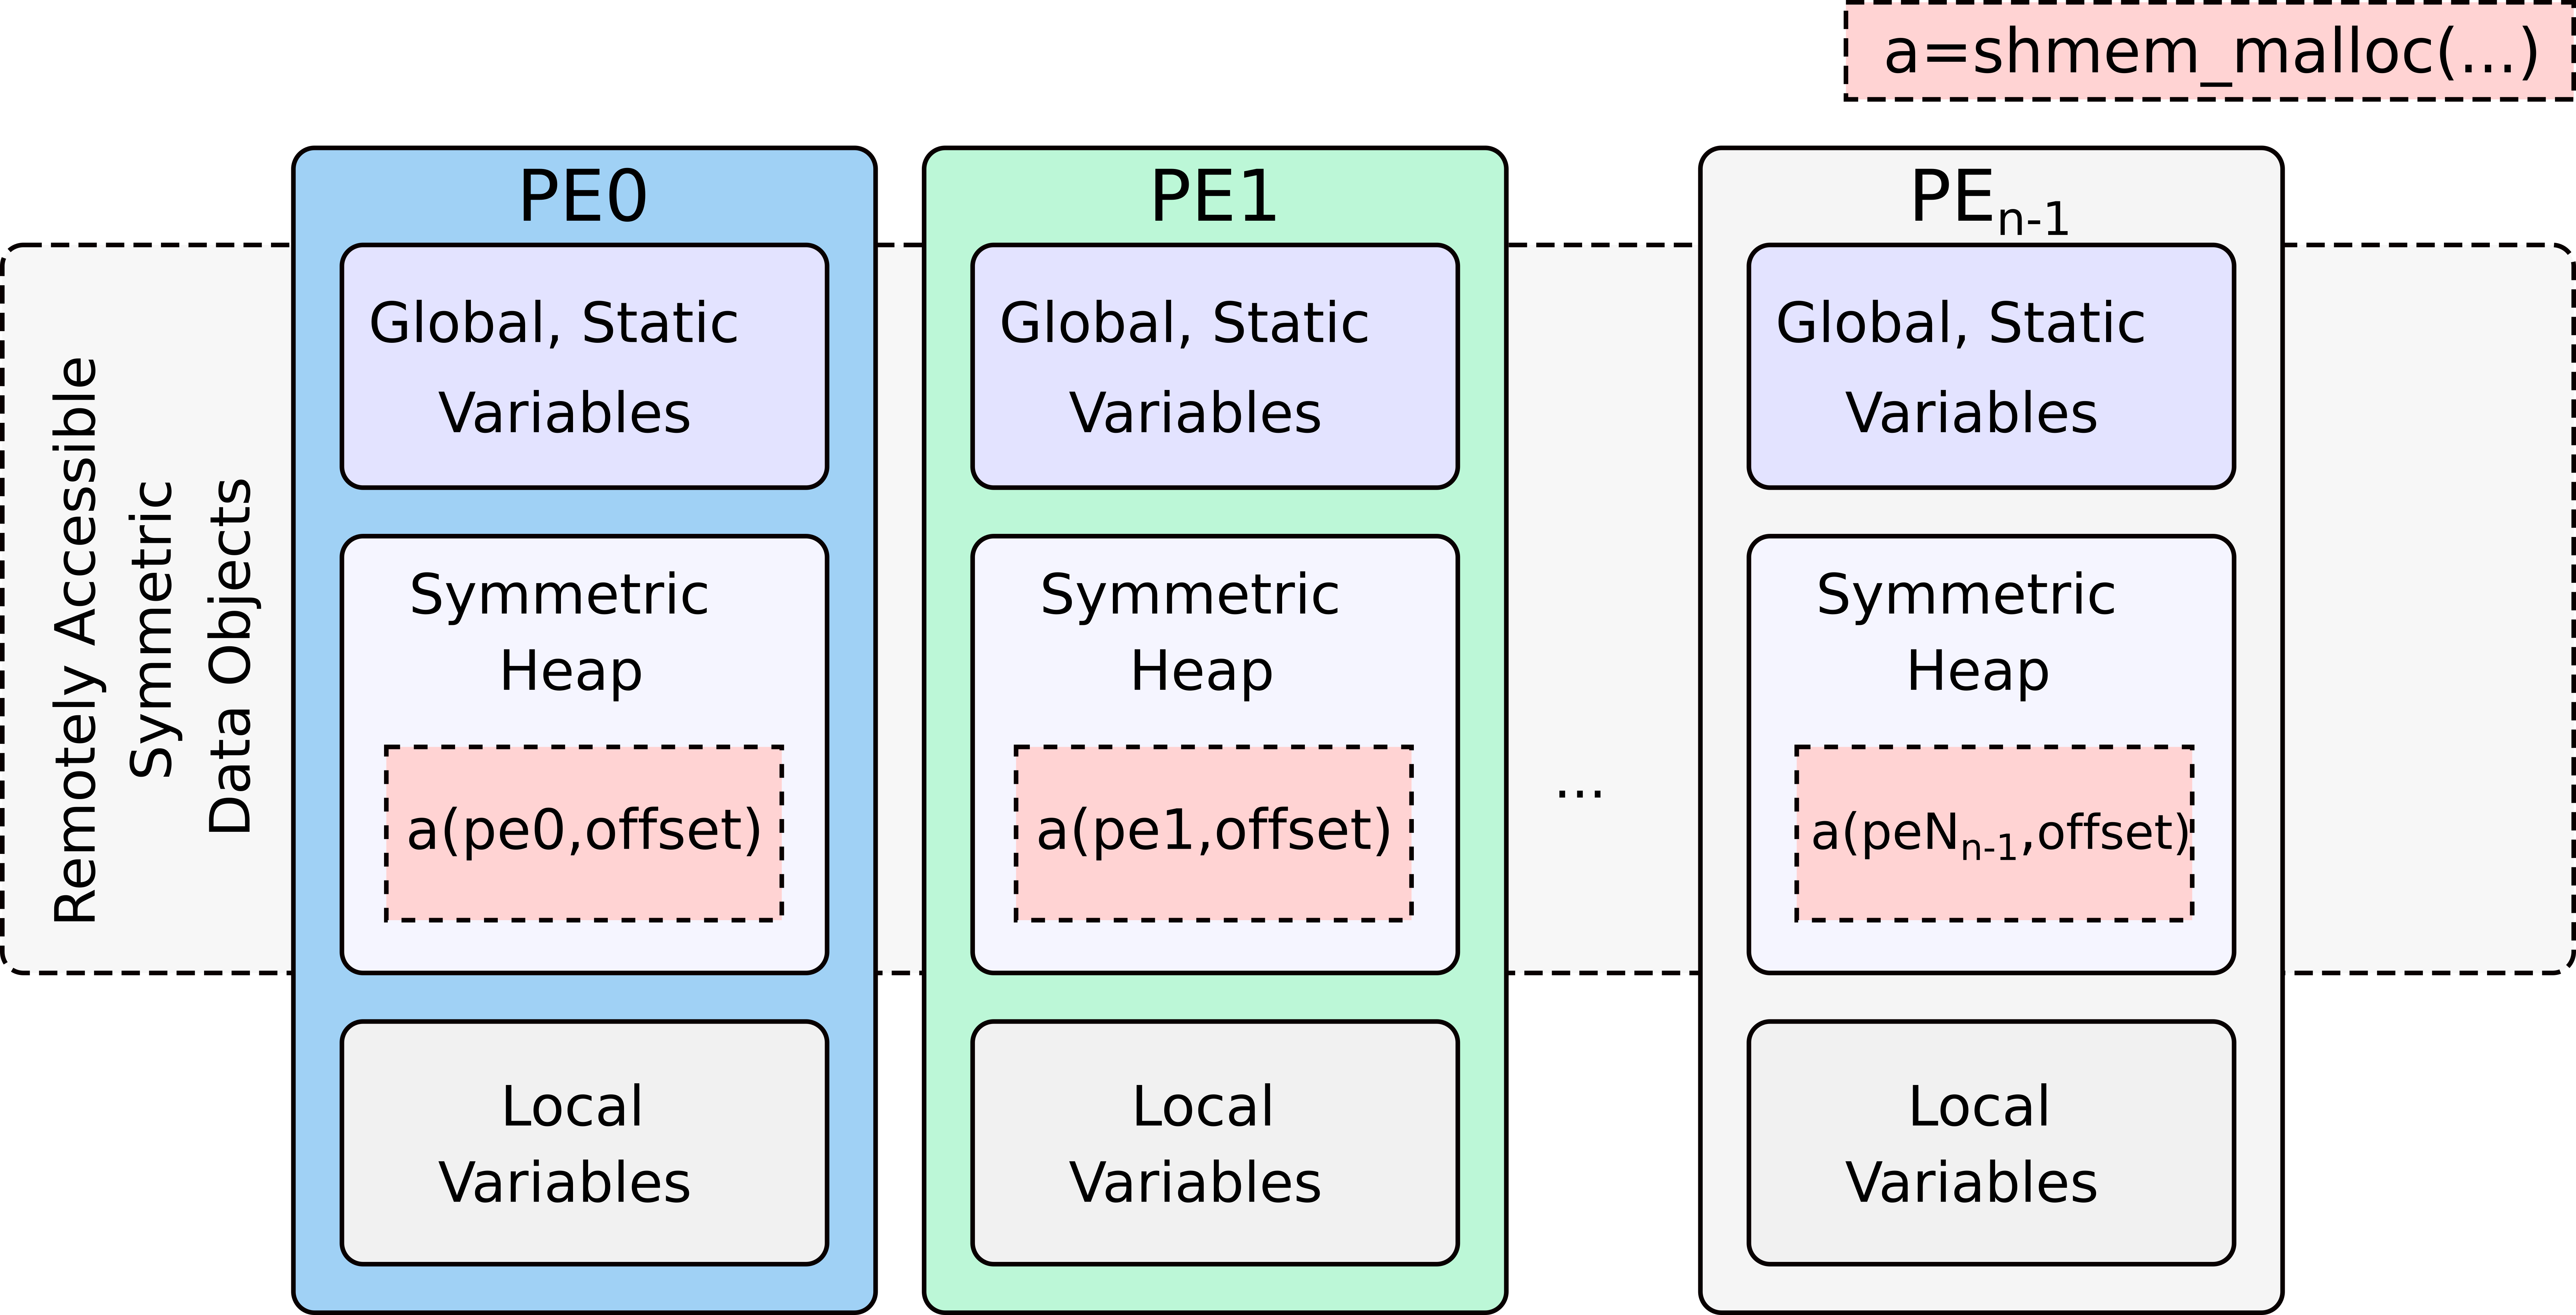
\includegraphics[width=0.8\textwidth]{figures/PGAS2}
  \end{center}
  \begin{itemize}
    \item Variable \texttt{a} is globally accessible through \texttt{Put} and \texttt{Get} operations,
    \texttt{PE} and \texttt{Offset} are used for global addressing.
    %\end{itemize}
  \end{itemize}
\end{frame}

%=============================================
%=============================================
%=============================================

\begin{frame}[fragile]{Remote Spaces: The PGAS Model}
  \vspace{10pt}
  \textbf{Different implementations, same conceptual API}
  \begin{itemize}
    \item OpenSHMEM
    \begin{itemize}
    \item void *shmem\_malloc(size\_t size);
    \item void shmem\_T\_p(T *dest, T value, int pe);
    \item TYPE shmem\_T\_g(T *src, int pe);
    \end{itemize}
    \item NVSHMEM
    \begin{itemize}
    \item void *nvshmem\_malloc(size\_t size);
    \item void nvshmem\_T\_p(T *dest, T value, int pe);
    \item TYPE nvshmem\_T\_g(TYPE *srct, int pe);
    \end{itemize}
    \item MPI One-Sided
    \begin{itemize}
    \item int *MPI\_Win\_allocate(size\_t size);
    \item int MPI\_Put(T *src, int count, MPI\_TYPE, int target\_pe,...);
    \item int MPI\_Get(T *target, int count , MPI\_TYPE, int source\_pe,...);
    \end{itemize}
  \end{itemize}
\end{frame}

%=============================================
%=============================================
%=============================================

\begin{frame}[fragile]{Remote Spaces: Namespace and API}
  \vspace{10pt}
  \textbf{Programming with Kokkos Remote Spaces: Vector Shift}
  \begin{itemize}
    \item Allocate a remote View
  \end{itemize}
  %\vspace{2pt}
  \begin{code}[keywords={RemoteSpace_t,RemoteView_t,Kokkos,View}]
  using RemoteSpace_t = Kokkos::Experimental::SHMEMSpace;
  Kokkos::View<T**,RemoteSpace_t> a("A",numPEs,myN);
  \end{code}
  %=============================================
  \pause
  \begin{itemize}
    \item Access global memory 
  \end{itemize}
  %\vspace{2pt}
  \begin{code}[keywords={RemoteSpace_t,RemoteView_t,Kokkos,View}]
  a(0,0) = 6; //Writes 6 to view a on PE 0 at offset 0
  a(1,8) = 3; //Writes 3 to view a on PE 1 at offset 8
  \end{code}
  %=============================================
  \pause
  %\vspace{2pt}
  \begin{itemize}
    \item Fence
  \end{itemize}
  \begin{code}[keywords={}]
  RemoteSpace_t().fence(); 
  \end{code}  
  %=============================================
    \pause
  %\vspace{2pt}
  \begin{itemize}
    \item Copy data to other memory space
  \end{itemize}
  \begin{code}[keywords={RemoteSpace_t,RemoteView_t,Kokkos,View,Experimental,deep_copy}]
  Kokkos::View<T**,Kokkos::HostSpace_t> a_h("A_h",1,myN);
  Kokkos::Experimental::deep_copy(a_h,a);
  \end{code}  
  %=============================================
\end{frame}

%=============================================
%=============================================
%=============================================

\begin{frame}[fragile]{Remote Spaces: Namespace and API}
  \vspace{10pt}
  \textbf{Vector Shift with Kokkos Remote Spaces}
    \vspace{4pt}
  \center
  \begin{center}
  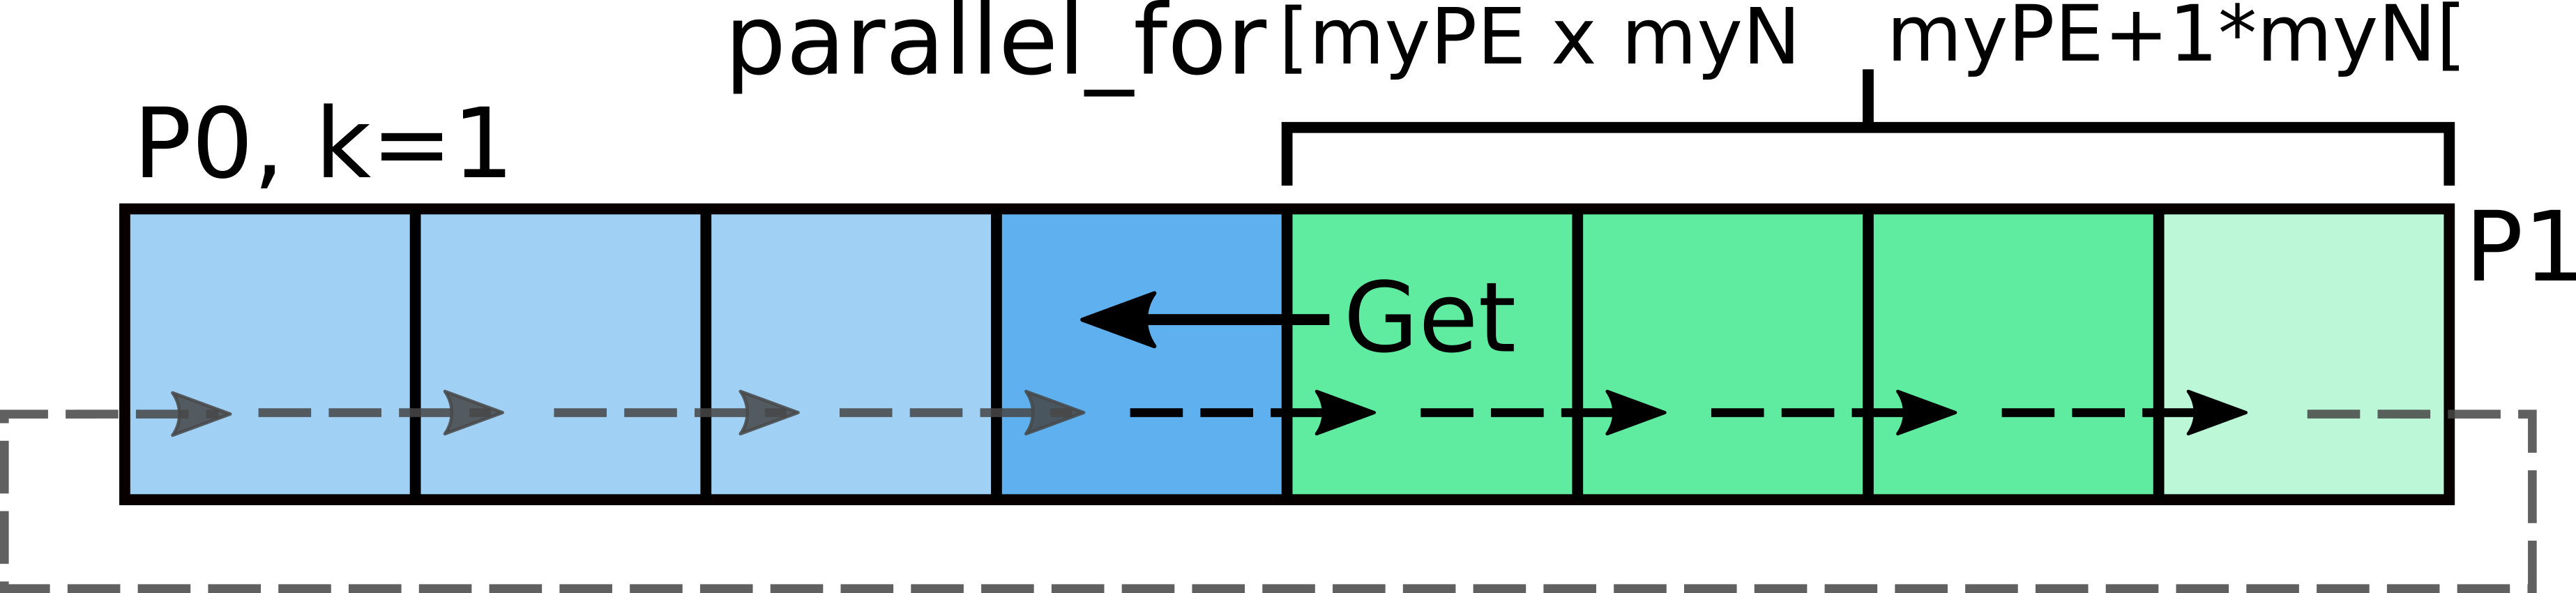
\includegraphics[width=0.50\textwidth]{figures/VectorShiftPGAS}
  \end{center}\
  \vspace{10pt}
  \begin{code}[keywords={RemoteSpace_t,RemoteView_t,parallel_for,Kokkos,View,Experimental,deep_copy, RangePolicy, KOKKOS_LAMBDA}]
  RemoteView_t a("A",numPEs,myN);
  RemoteView_t b("B",numPEs,myN);

  Kokkos::parallel_for("Shift",Kokkos::RangePolicy<>
  (myPE*myN,(myPE+1)*myN), KOKKOS_LAMBDA(const int i) { 
    int j = i+k; //Shift
    b((j/myN)%numPEs, j%myN) = a(myPE, i);
  });

  RemoteSpace_t().fence(); 
  \end{code}
\end{frame}

%=============================================
%=============================================
%=============================================

\begin{frame}[fragile]{Sparse Communication Patterns}
  \textbf{Example Sparse Matrix Multiply $y = A*x$:}
  Sparse Matrix Representation in Compressed Row Storage (CRS):
  \begin{itemize}
    \item Store non-zero matrix elements sorted by occurence.
    \item Store the actual column index of each value.
    \item Store the offsets of where each row begins.
  \end{itemize}
  \vspace{3pt}
  %=============================================
  \pause
    \textit{Single Node Implementation:}
    \begin{code}[keywords={for,RemoteSpace_t,RemoteView_t,parallel_for,Kokkos,View,Experimental,deep_copy,RangePolicy, KOKKOS_LAMBDA}]
      Kokkos::parallel_for("SPMV",nrows, KOKKOS_LAMBDA(int row) {
      for(j=A.row_offset(row); j< A.row_offset(row+1); j++)
      y(row) += A.val(j)* x(A.idx(j));
      });
    \end{code}\\
  %=============================================
  \pause

    \begin{columns}[t,onlytextwidth]
    \column{.7\textwidth}
     How to distribute data:
    \begin{itemize}
       \item The matrix is distributed by rows.
       \item The vectors are distributed by elements.
    \end{itemize}
    \textbf{Problem:$A.idx(j)$ may be on a remote node!}
    \column{.3\textwidth}
    \begin{center}
      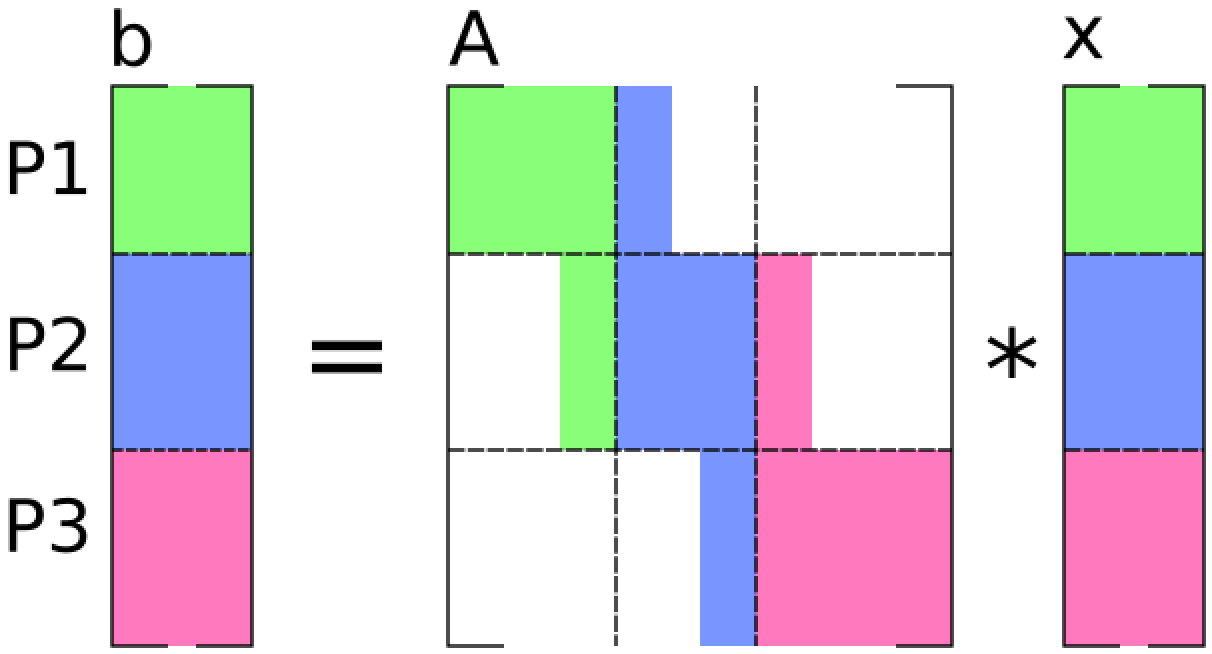
\includegraphics[width=1\textwidth]{figures/MatVecPGAS}
    \end{center}
  \end{columns}
\end{frame}

%=============================================
%=============================================
%=============================================

\begin{frame}[fragile]{SPMV in MPI}
    \textbf{MPI based SPMV needs a lof setup:}
  \begin{itemize}
    \item Find all values of A.idx(j) outside this ranks owned range.
    \item Find the ranks of each of those values which own them.
    \item Create for each of those ranks the list of indicies needed.
    \item Send the list to each rank, where it becomes the send\_list.
  \end{itemize}
  \vspace{5pt}
  \textbf{The data structures (Using View of Views (VoV)):}
  \begin{itemize}
    \item num\_recv\_ranks: Number of ranks you need data from.
    \item num\_send\_ranks: Number of ranks you need to send data too.
    \item recv\_buffers (2D VoV): list of recv buffer for each rank
    \begin{itemize}
      \item subviews into the end of x beyond owned elements.
    \end{itemize}
    \item send\_buffers (2D VoV): list of send buffer for each rank
    \item send\_lists (2D VoV): list of indicies to send to each rank
  \end{itemize}
\end{frame}

%=============================================
%=============================================
%=============================================

\begin{frame}[fragile]{SPMV in MPI}
\textbf{Code Skeleton for SPMV in MPI}
  \begin{code}[keywords={MPI_Irecv,MPI_Isend,MPI_Waitall,parallel_for,fence, Kokkos}]
    // Post all the recvs
    for(int i=0; i<num_recv_ranks; i++) {
      MPI_Irecv(recv_buffers(i).data(),nrecv(i)...);
    }
    // Pack send buffers and send
    for(int i=0; i<num_send_ranks; i++) {
      // Get the send buffer and list for this rank
      auto sb = send_buffer(i);
      auto sl = send_list(i);
      // Pack the data
      Kokkos::parallel_for(nsend(i),KOKKOS_LAMBDA(int j) 
        { sb(i) = x(sl(j)); });
      Kokkos::fence();
      // Send the data
      MPI_Isend(sb.data(),nsend(i),...);
    }
    // Wait for all the communication to be done
    MPI_Waitall(...);
    // Run the local code
    parallel_for("SPMV",...);
  \end{code}
\end{frame}

%=============================================
%=============================================
%=============================================

\begin{frame}[fragile]{SPMV in PGAS}
  \textbf{Sparse communication with PGAS is easy!}
  \begin{itemize}
    \item Only \texttt{x} is distributed!
    \item Simply keep using global indicies in A.idx
    \item Compute PE and offset with div and mod for accessing \texttt{x}
  \end{itemize}

  \begin{code}[keywords={for,MPI_Irecv,MPI_Isend,MPI_Waitall,parallel_for,fence, Kokkos}]
  Kokkos::parallel_for("SPMV",my_nrows, KOKKOS_LAMBDA(int row) {
    for(j=A.row_offset(row); j< A.row_offset(row+1); j++) {
      int idx_j = A.idx(j);
      int pe = idx_j/N_local;
      int k = idx_j%N_local;
      y(row) += A.val(j)*x(pe,k);
    }
  });
  \end{code}\\
  Remember the MPI Skeleton? This is the skeleton in PGAS:
  \begin{code}
    parallel_for("SPMV",...);
  \end{code}
\end{frame}

%=============================================
%=============================================
%=============================================

\begin{frame}{Remote Spaces: CGSolve Results}
  \textbf{CGSolve with Kokkos Remote Spaces}
  \vspace{5pt}
  \begin{itemize}
    \item\small Lassen Supercomputer (LLNL), IBM Power9, 4x NVidia Volta GPUs
  \end{itemize}
  \begin{columns}[t,onlytextwidth]
    \column{.5\textwidth}
    \begin{center}
      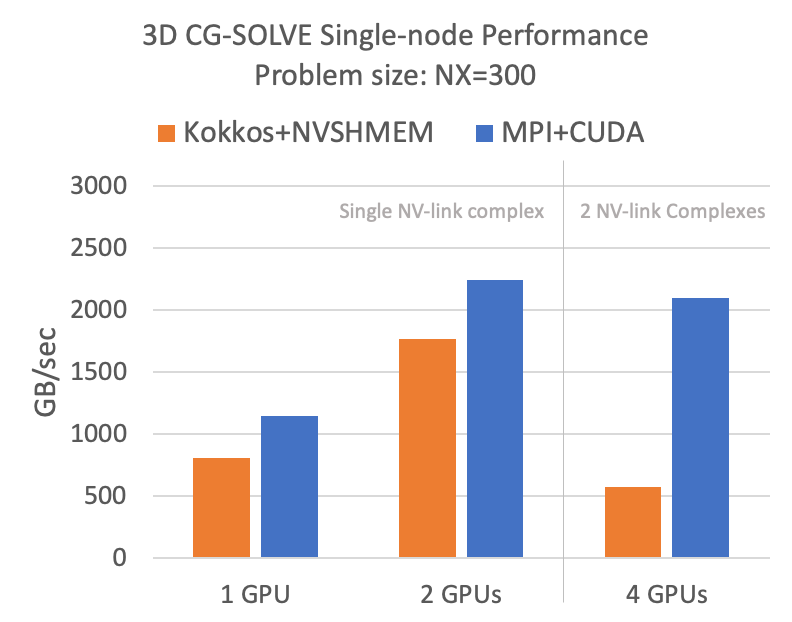
\includegraphics[width=0.99\textwidth]{figures/PGAS_CGSolve_Perf}
    \end{center}
    \column{.5\textwidth}
    \begin{center}
      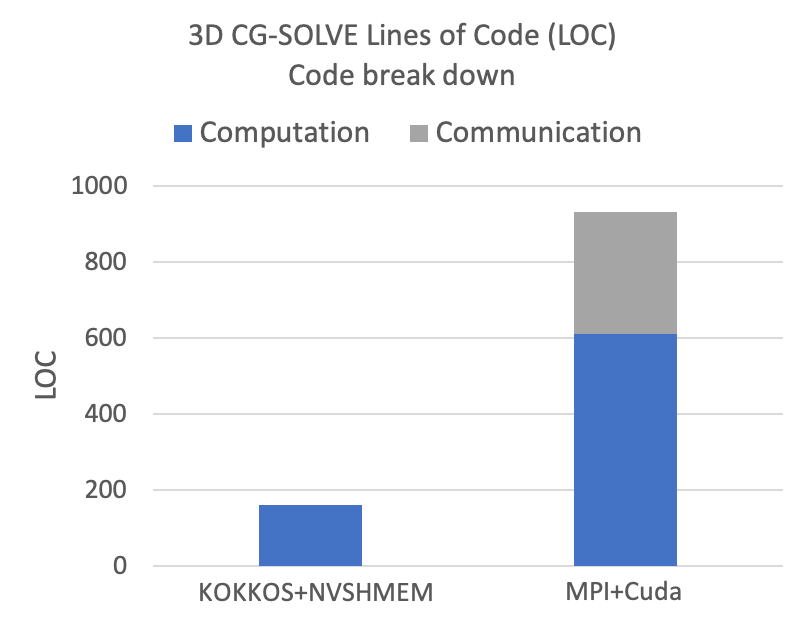
\includegraphics[width=0.99\textwidth]{figures/PGAS_CGSolve_LOC}
    \end{center}
  \end{columns}
\end{frame}

%=============================================
%=============================================
%=============================================

\begin{frame}{Remote Spaces: Code and Configuration}
  \vspace{6pt}
  \textbf{Get it on GitHub}
  \begin{itemize}  
  \item\url{https://github.com/kokkos/kokkos-remote-spaces}
  \end{itemize}
  \vspace{6pt}
  \textbf{Configuration Example}
  \begin{itemize}
    \item\textbf{NVSHMEM}: \small\texttt{cd \$(kokkos\_remote\_spaces) \\
  cmake . -DKokkos\_DIR=\$(KOKKOS\_HOME)/install -DCMAKE\_CXX\_COMPILER=mpicxx  -DNVSHMEM\_ROOT=\$(NVSHMEM\_HOME)/install -DKokkos\_ENABLE\_NVSHMEMSPACE=ON}
  \item\textbf{SHMEM}: \small\texttt{-DKokkos\_ENABLE\_SHMEMSPACE=ON}
  \item\textbf{MPI One-Sided:}\small\texttt{-DKokkos\_ENABLE\_MPISPACE=ON}
  \end{itemize}
  \vspace{8pt}
  % \begin{block}{Important Point}
    \textbf{Note:} Setting the \texttt{-DKokkos\_ENABLE\_\{SPACE\}} CMAKE flag sets \texttt{Kokkos::Experimental::DefaultRemoteMemporySpace} to the given \textbf{PGAS backend}.
  %\end{block}
\end{frame}

%=============================================
%=============================================
%=============================================

\begin{frame}[fragile]{Exercise: Vector-Shift}
\textbf{Exercise: Implementing a Distributed Vector-Shift}
  \vspace{10pt}
  \begin{itemize}
    \item Location: \ExerciseDirectory{pgas\_vectorshift}
    \item Compile and run with one and two ranks using SHMEM (CPUs) or NVSHMEM (GPUs)
  \end{itemize}
  
  \begin{code}
    mkdir build && cd build
    cmake . -DKokkosRemote_ROOT=<path-to-Kokkos-Remote-Spaces>/install -DCMAKE_CXX_COMPILER=mpicxx
    cmake .. && make
    # Run exercise
    mpiexec -np 2 ./vectorshift
  \end{code}
\end{frame}

%=============================================
%=============================================
%=============================================

\begin{frame}{Remote Spaces: Summary}
\textbf{Summary: Kokkos Remote Spaces}
\vspace{10pt}
\begin{itemize}
   \item Adds distributed shared memory to Kokkos.
   \item View-templating defines memory space (SHMEM, NVSHMEM or MPI One-Sided).
   \item View \texttt{()-operator} implements the \texttt{Put/Get semantic}.
   \item Use \texttt{deep\_copy(...)} to move data between memory spaces.
\end{itemize}
\end{frame}

%=============================================
%=============================================
%=============================================


\begin{frame}{Module 6 Summary}
\textbf{Simple MPI and Kokkos Interaction is easy!}
\begin{itemize}
  \item Simply pass \texttt{data()} of a View to MPI functions plus its size.
  \begin{itemize}
    \item But it better be a contiguous View!
  \end{itemize}
  \item Initialize Kokkos after MPI, and finalize it before MPI
\end{itemize}

\vspace{10pt}
\textbf{Overlapping communication and computation possible}
\begin{itemize}
  \item Use Execution Space instances to overlap packing/unpacking with other computation.
  \item Order operations to maximize overlapping potential. 
\end{itemize}
\end{frame}

\begin{frame}[fragile]{Module 6 Summary}
\textbf{Fortran Language Compatibility Layer}
\begin{itemize}
  \item Initialize Kokkos from Fortran via \texttt{kokkos\_initialize} and \texttt{kokkos\_finalize}
  \item \texttt{nd\_array\_t} is a representation of a \texttt{Kokkos::View}
  \item Create \texttt{nd\_array\_t} from a Fortran array via \texttt{to\_nd\_array}
  \item Allocate \texttt{Kokkos::DualView} in Fortran with \texttt{kokkos\_allocate\_dualview}
\end{itemize}


  \vspace{10pt}
  \textbf{The Python Interop}
  \begin{itemize}
    \item Initialize and Finalize Kokkos from Python
    \item Create Views from Python
    \item Alias Kokkos Views with NumPy arrays
    \item \textbf{This is in pre-release: ask us for access.}
  \end{itemize}
\end{frame}

\begin{frame}{Module 7: Outlook (08/28)}
    \vspace{-3pt}
	\textbf{Clang-Tidy Static Analysis}
	\begin{itemize}
        \item {Getting Kokkos specific warnings in your IDE}
	\end{itemize}
	
	\vspace{5pt}
	\textbf{Kokkos Tools}
	\begin{itemize}
		\item {Debugging}
		\item {Profiling}
                \item {Tuning}
	\end{itemize}

	\vspace{5pt}
	\textbf{Custom and 3rd party tools}
	\begin{itemize}
		\item {How to write distributed code using a global arrays like interface}
	\end{itemize}

	\vspace{5pt}
	\textbf{Don't Forget:} Join our Slack Channel and drop into our office hours on Tuesday.
	
	\vspace{5pt}
	\textbf{Updates at:} \href{https://kokkos.link/the-lectures-updates}{kokkos.link/the-lectures-updates}
	
	\vspace{5pt}
	\textbf{Recordings/Slides:} \href{https://kokkos.link/the-lectures}{kokkos.link/the-lectures}

\end{frame}

\end{document}

